\documentclass[12pt,a4paper,oneside]{book}
\usepackage[utf8]{inputenc}
\usepackage[ngerman]{babel}
\usepackage[T1]{fontenc}
% s. src/config/acros.tex
%\usepackage[]{acronym}


\usepackage{acro}

\acsetup{
  index, 
  only-used=false,
  list-style=extra-tabular
}


 \DeclareAcronym{SRP}{
   short = {SRP},
   long = {Single Responsibility Principle}
 }
 \DeclareAcronym{OCP}{
   short = {OCP},
   long = {Open-Closed Principle}
 }
 \DeclareAcronym{LSP}{
   short = {LSP},
   long = {Liskov Substitution Principle}
 }
 \DeclareAcronym{ISP}{
   short = {ISP},
   long = {Interface Segregation Principle}
 }
 \DeclareAcronym{DIP}{
   short = {DIP},
   long = {Dependency Inversion Principle}
 }
 \DeclareAcronym{REP}{
   short = {REP},
   long = {Reuse/Release Equivalence Principle}
 }
 \DeclareAcronym{CCP}{
   short = {CCP},
   long = {Common Closure Principle}
 }
 \DeclareAcronym{CRP}{
   short = {CRP},
   long = {Common Reuse Principle}
 }
 \DeclareAcronym{ADP}{
   short = {ADP},
   long = {Acyclic Dependency Principle}
 }
 \DeclareAcronym{DAG}{
   short = {DAG},
   long = {Directed Acyclic Graph}
 }
 \DeclareAcronym{SDP}{
   short = {SDP},
   long = {Stable Dependency Principle}
 }
 \DeclareAcronym{SAP}{
   short = {SAP},
   long = {Stable Abstraction Principle}
 }
 \DeclareAcronym{IoC}{
   short = {IoC},
   long = {Inversion of Control}
 }
 \DeclareAcronym{DI}{
   short = {DI},
   long = {Dependency Injection}
 }
 \DeclareAcronym{GUI}{
   short = {GUI},
   long = {Graphical User Interface}
 }
 \DeclareAcronym{JRE}{
   short = {JRE},
   long = {Java Runtime Environment}
 }
 \DeclareAcronym{JPQL}{
   short = {JPQL},
   long = {Java Persistence Query Language}
 }
 \DeclareAcronym{JSON}{
   short = {JSON},
   long = {JavaScript Object Notation}
 }
 \DeclareAcronym{WAR}{
   short = {WAR},
   long = {Web Archive}
 }
 
 


% Hauptdatei des Projektes. Von hier aus werden die anderen Seiten eingebunden
\input{src/config/konfiguration.tex}
% Nützliches
%https://stackoverflow.com/questions/3175105/writing-code-in-latex-document
\newcommand{\code}[1]{\texttt{#1}}

\newcommand{\dqs}[1]{\textquotedbl #1\textquotedbl\xspace}
\newcommand{\citeauth}[1]{\citet{#1}}
\newcommand{\refSec}[1]{s. Kapitel~\ref{#1}}
\newcommand{\refSecns}[1]{Kapitel~\ref{#1}}
\newcommand{\refAbb}[1]{s. Abbildung~\ref{#1}}
\newcommand{\refAbbns}[1]{Abbildung~\ref{#1}}
\newcommand{\refLis}[1]{s. Listing~\ref{#1}}
\newcommand{\refLisns}[1]{Listing~\ref{#1}}
\newcommand{\refTab}[1]{s. Tabelle~\ref{#1}}
\newcommand{\refTabns}[1]{Tabelle~\ref{#1}}
\newcommand{\refLst}[1]{s. Listing~\ref{#1}}
\newcommand{\refLstns}[1]{Listing~\ref{#1}}

% Kurzformen
\newcommand{\zb}{z.\,B.\xspace}
\newcommand{\ua}{u.\,a.\xspace}
\newcommand{\oge}{o.\,g.\xspace}
\newcommand{\dah}{d.\,h.\xspace}
\newcommand{\bzw}{bzw.\xspace}
\newcommand{\bzgl}{bzgl.\xspace}
\newcommand{\ggf}{ggf.\xspace}
\newcommand{\bspw}{beispielsweise\xspace}

% Silbentrennung
\hyphenation{Funk-tions-be-reich}
\hyphenation{An-wen-der-be-treu-ung}
\hyphenation{Prüf-spe-zi-fi-ka-tion}
\hyphenation{Soft-ware-pro-jekt}
\hyphenation{Soft-ware}
\hyphenation{Per-so-nal-wachs-tum}
\hyphenation{le-dig-lich}
\hyphenation{Sys-tem-as-pek-te}
\hyphenation{Ver-zö-ger-ung-en}
\hyphenation{under-stand-abi-lity}
\hyphenation{Än-de-rung-en}
\hyphenation{da-rü-ber}







% Für Kopf und Fußzeile: https://esc-now.de/_/latex-individuelle-kopf--und-fusszeilen/?lang=en
\usepackage[
  headsepline, plainheadsepline,
  footsepline, plainfootsepline
]{scrlayer-scrpage}
\pagestyle{scrheadings}
\clearscrheadfoot

\ihead*{\itshape\leftmark}
\ifoot*{\today}
\ofoot*{\pagemark}


\input{src/pdfa.tex}

\begin{document}

\pagenumbering{roman}
\setcounter{page}{2}


\chapter*{Zusammenfassung}
\markboth{Abstract}{}
\label{sec:Abstract}

In dieser Arbeit wird geprüft, welche Rolle eine saubere Softwarearchitektur für eine erweiter"= und wartbare Software spielt. Dabei wird die Transaktionserfassung als Teil des Systems WBS Alarm analysiert, bewertet und überarbeitet. WBS Alarm ist eine Open Source Anwendung zur Kleiderverwaltung der freiwilligen Feuerwehr in Eschenstruth. Aus den gewonnen Erkenntnissen werden Lösungen modelliert und beurteilt, ob die empfohlenen Vorgehensweisen einen Beitrag zu wartbarer Software leisten. Dabei wird festgestellt, dass eine Restrukturierung eines Teilsystems neue Aufgaben im Gesamtsystem schafft und dieses somit bei Restrukturierung von Teilsystemen immer mit in Betracht gezogen werden sollte.

{\let\clearpage\relax\chapter*{Abstract}}

\begin{otherlanguage}{british}
This thesis examines the role of a clean software architecture for an extensible and maintainable software. Thereby the transaction capture as part of the system WBS Alarm is analyzed, evaluated and revised. WBS Alarm is an open source application for the clothing management of the voluntary fire brigade in Eschenstruth. Based on the gained knowledge, solutions are modelled and it is assessed whether the recommended procedures contribute to maintainable software. It is stated that restructuring a subsystem creates new tasks in the overall system and that this should therefore always be taken into account when restructuring subsystems.
\end{otherlanguage}


%Inhaltsverzeichnis
\setcounter{tocdepth}{2}
\tableofcontents

\newpage

\pagenumbering{arabic}
  
% Abstand nach Absätzen
\setlength{\parskip}{0.3cm}

% falls man lieber eine Datei pro Kapitel bevorzug, kann man dies auch einfach realisieren, indem man diese wie folgt einbindet
\chapter{Einleitung}
\markboth{Einleitung}{}
\label{ch:Einleitung}

Während des Softwareprojekts im Rahmen des Studiums der Sozialinformatik wurde eine Open Source Software namens WBS Alarm entwickelt, welche die Kleiderkammer der freiwilligen Feuerwehr in Eschenstruth digitalisieren sollte. Das Projekt erfolgte in vier Phasen á zwei Monaten, die sich insgesamt über zwei Jahre hinweg verteilten. In der ersten Phase wurden die Anforderungen aufgenommen und das Vorgehen geplant. Dabei wurde auch festgelegt, dass es sich um eine Webanwendung handeln soll, damit die Mitglieder der Feuerwehr auch mobil arbeiten können. In der zweiten Phase wurde die Administration erstellt, in der alle notwendigen Daten erfasst werden können, die für eine Kleiderbuchung benötigt werden. Zudem wurde das System gegen unbefugten Zugriff mit einem Login gesichert. In der dritten Phase wurde die zentrale Geschäftslogik entwickelt, bei der Transaktionen zwischen Ortsteilen gebucht werden können. Dabei wurde die Software auch auf einem Server für die Kunden bereitgestellt und veröffentlicht. In der vierten Phase wurden Berichte hinzugefügt, ein Versand von Statusnachrichten per E-Mail eingerichtet und die Struktur der Oberfläche angepasst.

In der dritten Phase sind einige Teile nicht zukunftsfähig entwickelt worden. Die Anforderungen haben mehr Zeit in Anspruch genommen als ursprünglich dafür geplant gewesen war, weshalb die Bearbeitungszeit für andere Teilaspekte des Projekts gekürzt werden musste. Dies betraf insbesondere die Transaktionserzeugung als zentralsten und komplexesten Teil der Geschäftslogik. 

In dieser Arbeit wird zunächst geprüft, inwieweit eine saubere Softwarearchitektur dabei helfen kann die Transaktionserzeugung wartbar und erweiterbar zu halten bzw. sie zu verbessern und diese Verbesserungen anschließend umgesetzt. 

In Kapitel~\ref{ch:Grundlagen} wird zunächst das Projekt WBS Alarm selbst vorgestellt und die Anforderungen an die Transaktionserzeugung definiert und erläutert. Zudem wird auf zwei Fallstudien Bezug genommen, in denen beschrieben wird, warum eine saubere Softwarearchitektur benötigt wird und wie dies für Weiterentwicklungen eine Rolle spielt. Danach werden Design- und Komponentenprinzipien, sowie ein Ansatz einer sauberen Softwarearchitektur aus aktueller Fachliteratur zusammengefasst, die für die Optimierung der Transaktionserfassung von Bedeutung sind.

Die zentrale Fragestellung lautet in dieser Arbeit: Kann anhand der Design- und Komponentenprinzipien die Struktur der Transaktionserfassung optimiert werden, sodass bei Anforderungsänderungen oder ‑erweiterungen diese effizient angepasst werden kann? In Kapitel~\ref{ch:Fragestellung} wird hierauf genauer eingegangen.

Im Kapitel~\ref{ch:Vorgehensweise} wird mit Hilfe von UML der Ausgangszustand modelliert. Dieser wird daraufhin anhand der erarbeiteten Grundlagen analysiert. Wenn sich in der Analyse ergeben sollte, dass gegen bestimmte Design- und Komponentenprinzipien verstoßen wurde, wird eine Anpassung erst mit UML geplant und dann entsprechend mit Java umgesetzt.

Die Erkenntnisse werden im Kapitel~\ref{ch:Auswertung} ausgewertet.

Schließlich wird in Kapitel~\ref{ch:Fazit} ein Fazit über die genannten Prinzipien gezogen und ob sich eine Umstrukturierung für das Projekt WBS Alarm gelohnt hat.
\chapter{Grundlagen}
\markboth{Grundlagen}{}
\label{ch:Grundlagen}

In diesem Kapitel wird zuerst auf das Projekt WBS Alarm eingegangen und die Anforderungen an die Erfassung der Transaktionen ausführlich beschrieben. Hier soll erläutert werden, welche Gedankengänge hinter den Anforderungen stecken. 

Danach werden zwei Fallstudien vorgestellt, die sich mit dem Kostenwachstum der Entwicklung und Wartung mit fortschreitenden Releases, also Veröffentlichungen eines Softwareprodukts, beschäftigt haben. Hier werden die wichtigsten Erkenntnisse aus den Fallstudien zusammengefasst.

Im Folgenden wird in Kapitel~\ref{sec:Softwarearchitektur} auf einzelne Details einer sauberen Softwarearchitektur eingegangen. In den Kapiteln~\ref{sec:Designprinzipien} und~\ref{sec:Komponentenprinzipien} werden einige Prinzipien für die Entwicklung leicht wart"= und erweiterbarer Software vorgestellt. 

\section{WBS Alarm}
\label{sec:wbs}

WBS Alarm ist ein Warenbestandssystem, das für die freiwillige Feuerwehr in Eschenstruth im Laufe des Studiums Sozialinformatik entwickelt wurde. Die Software entstand aus dem Bedürfnis, einen Überblick über den aktuellen Bestand an Kleidung und ihrer Verteilung zu schaffen. Dies wurde zuvor auf externen Datenträgern wie Tafeln, Zetteln und als Microsoft Excel Tabelle auf einem USB Stick verteilt. Diese Variante war auf Dauer von den Mitgliedern der Feuerwehr nicht mehr zu handhaben, da die Informationen mit der Zeit auseinandergeflossen sind und der Überblick schwand. Daher sollte eine Software entwickelt werden, die diesen Missstand aufhebt. Über einen Zeitraum von zwei Jahren wurde das Projekt abgeschlossen und ist mittlerweile in einem produktiven Zustand. 

Im Wesentlichen wird in WBS Alarm ein Träger der freiwilligen Feuerwehr verwaltet. Im Beispiel von Eschenstruth wäre dies die Gemeinde Helsa. Unter dem Träger werden die Anwender, Zielorte und Kleidungsstücke verwaltet. Bei der Anlage eines Trägers werden vier Zielorte angelegt: Wareneingang, Lager, Wäscherei und Aussonderung. Der Wareneingang hat als Sonderstellung keine verwaltbaren Bestände, da alle Einkäufe darüber gebucht werden. Der Wareneingang selbst steht aber nicht als Zielort für Buchungen zur Verfügung. Es steht den Administrator*innen die Option offen, in WBS Alarm eigene Wareneingänge zu erstellen. Somit könnten Lieferanten abgebildet werden. Die Wäscherei ist aus der Anforderungsanalyse mit der freiwilligen Feuerwehr entstanden.

Die Transaktionserfassung ist der zentrale Punkt der Software und stellt als komplexesten Teil den Kern des Systems dar. Die Anforderungen an eine Transaktion werden wie folgt definiert: 

\begin{itemize}
\item Ein Anwender kann nur für seinen eigenen Träger eine Transaktion erfassen.
\item Eine Transaktion hat immer genau einen Ursprungsort und einen Zielort.
\item Der Ursprungsort und der Zielort müssen unterschiedlich sein.
\item Der Urspungsort und der Zielort gehören zum Träger des Anwenders.
\item Eine Transaktion umfasst mindestens eine Position. 
\item Eine Position besteht aus einem Kleidungsstück und dessen Anzahl.
\item Ein Kleidungsstück darf nur in einer Position pro Transaktion vermerkt sein.
\item Das verbuchte Kleidungsstück ist im Ursprungsort in der gewünschten Anzahl vorhanden --- dies gilt sofern es sich beim Ursprungsort nicht um den Wareneingang handelt, über den neue Kleidungsstücke aufgenommen werden. 
\item An den Wareneingang darf nicht gebucht werden.
\item Die Orte müssen für die Erfassung gesperrt sein, \dah ein Ort, dessen Bestand durch einen administrativen Anwender initial erfasst worden ist, muss für weitere Änderungen gesperrt werden. Somit wird eine Manipulation der Bestandswerte vermieden. Wenn bei einer Inventur Missstände festgestellt werden, muss eine Korrektur über die Buchungsschnittstelle erfolgen.
\end{itemize}

Diese Anforderungen muss eine Transaktion erfüllen, um in WBS Alarm verbucht zu werden.


\section{Kostenwachstum je Release}
\label{sec:Kostenwachstum}

In einer Fallstudie hat \citeauth{martin2018} das Kostenwachstum für jedes erbrachte Release untersucht. Dabei hat er aus einem untersuchten Unternehmen, das anonym bleiben wollte, den Lebenszyklus eines marktführenden Softwareprodukts analysiert. Der Umfang des Entwicklungsteams hat über acht Releases signifikant zugenommen (\refAbb{fig:staff_rel}), die Anzahl der Zeilen an Quellcode hat sich ab einem gewissen Punkt aber nicht mehr stark vermehrt (\refAbb{fig:kloc_rel}). Die Produktivität des Entwicklerteams (\refAbb{fig:prod_rel}) fiel schon ab dem vierten Release mit jedem weiteren Release immer weiter gegen Null. Für das Entwicklerteam ist das frustrierend, da alle Bemühungen das Produkt zu erweitern, den Aufwand und die Anstrengungen für zukünftige Produktversionen vermehrt \citep[vgl.][5\psqq]{martin2018}. 

Bei der Analyse der Probleme ist \citeauth{martin2018} auf zwei wesentliche Faktoren gestoßen. Zum einen musste das Produkt schnell auf den Markt gebracht werden. Den Quellcode strukturieren und aufräumen könne aus Sicht der Projektleitungen danach erledigt werden und wurde entsprechend verschoben. Diese Vorgehensweise wurde aber weiterhin durchgeführt, da der Marktdruck nicht nachgelassen hat. Somit wurde die Wartung und Pflege des vorhandenen Quellcodes immer weiter aufgeschoben. Der andere Faktor war die Annahme, dass unordentlicher Code auf kurze Sicht einen Geschwindigkeitsvorteil bringt und alles andere langfristig nur aufhält \citep[vgl.][10]{martin2018}.

Der beste Weg die Lebensdauer von Softwareprodukten gewinnbringend zu erhöhen ist laut \citeauth{martin2018}, der Qualität der eigenen Softwarearchitektur mehr Bedeutung beizumessen und ernster zu nehmen \citep[vgl.][12]{martin2018}.


\begin{figure}
  \centering
  \includegraphics[width=.6\textwidth]{res/staff_releases.jpg}
   \caption{Personalwachstum im Entwicklungsbereich mit jedem Release \citep[][5]{martin2018}.}
   \label{fig:staff_rel}
\end{figure}


\begin{figure}
  \centering
  \includegraphics[width=.6\textwidth]{res/kloc_releases.jpg}
   \caption{Anzahl Zeilen an Quellcode mit jedem Release \citep[][6]{martin2018}.}
   \label{fig:kloc_rel}
\end{figure}


\begin{figure}
  \centering
  \includegraphics[width=.6\textwidth]{res/productivity_releases.jpg}
   \caption{Produktivität des Entwicklungsteams mit jedem Release \citep[][8]{martin2018}.}
   \label{fig:prod_rel}
\end{figure}


In einer weiteren Fallstudie setzt \citeauth{Ogheneovo2014} die Komplexität und die Instandhaltungs"= und Evolutionskosten von Software in Verbindung. Da Software sich über die Zeit weiter entwickelt (\textit{Evolution}), wird sie gleichzeitig auch komplexer, wenn nicht der Quellcode restrukturiert wird um die Komplexität zu verringern. Dies kann \zb als Ergebnis einer Instandhaltungsmaßnahme sein. Unter Evolution einer Software kann die Erweiterung von Funktionen verstanden werden, die einen weiteren Nutzerkreis ansprechen soll. Auch der Einsatz von neuen Technologien, um neuen Funktionen gerecht zu werden, fallen als Evolutionskosten an \citep[vgl.][3]{Ogheneovo2014}.

%\textquote[{\cite[][3]{Ogheneovo2014}}]{Software maintenance and evolution of systems was first proposed by Lehman in 1969 [11]. Lehman notes that systems continue to evolve over time. As a result, they become more complex unless some action such as code refactoring is adopted to reduce the complexity that may arise as a result of maintenance. [...] 
%The software value can be enhanced by expanding the customer base, meeting additional requirements, thus making the software more easier to use, more efficient, more reliable, and employing new technology to cater for the new features that may be introduced to these technologies. Software evolution plays an important role in software maintenance process. Most development effort and expenditure is allocated to the evolution and update of existing versions of software. Software is ceaselessly changed—maintained, evolved and updated—more often than it is written, and changing software is extremely costly.}.

In die Instandhaltungsphase fallen 60 bis 70\% der Aufwände. Damit umfasst sie den größten Teil der Entwicklung und auch einen Großteil der kompletten Lebenszykluskosten \citep[vgl.][3]{Ogheneovo2014}.

%\textquote[{\cite[][3]{Ogheneovo2014}}]{Barry et al. [14] notes that about 60 to 70\% effort is expended on maintenance phase of software development life cycle. It therefore suffix to say that software maintenance activities span a system’s productive life cycle and consume a major part of the total life cycle costs of the system. The software maintenance process can last for years or even decades after development process [15]. Therefore, there is need for effective planning in order to address the scope of software maintenance, the tailoring of the post delivery/deployment, the designation of who will pro- vide maintenance, and an estimation of the life-cycle costs. Software maintenance takes more effort than all the other phases of software life cycle.}.

Ein Faktor, der die Instandhaltungskosten verringern kann, ist die Modularisierung der Software. Hiermit werden Teile der Software in einzelne Module aufgeteilt und wieder neu miteinander verbunden. Durch die logische Aufteilung des Softwaredesigns kann die Komplexität verringert und die einzelnen Module wartbarer gemacht werden. In der Entwicklung spielt das Konzept der Modularisierung eine wichtige Rolle. \textit{Microsoft} hat mehr als drei Jahre gebraucht um \textit{Windows Vista} letztendlich zu veröffentlichen. Hier waren die Module logisch so groß aufgebaut, dass die Programmkomplexität anstieg. Mit jedem Patch und jeder Verbesserung wurde es schwieriger neue Funktionalitäten einzuführen. Deshalb mussten Untermodule geschaffen werden, welche die Komplexität verringerten. Durch die fehlende Strukturierung und Modularisierung des Programmcodes verzögerte sich die Markteinführung von \textit{Windows Vista} \citep[vgl.][8\psq]{Ogheneovo2014}.

%\textbf{Factors Affecting Software Maintenance Costs}
%\textquote[{\cite[][8\psq]{Ogheneovo2014}}]{Modularity: Modularity is the degree to which system’s components may be separated or recombined. In modular programming, modularity refers to the compartmentalization and inter-relation of the parts of a software system. It is the logical partitioning of software design that allows complex software to be manageable for the purpose of implementation and maintenance. This logic may be based on related functions, implementation considerations, data links etc. Baldwin and Clark [41] in their theory note that modular architectures add value to system designs by creating options to improve the system by substituting or experimenting on individual modules.
%The concept of modularity is very important in software development and maintenance. According to [42], it took Microsoft more than three years of delay before they finally released Windows Vista. This was attributed to the presence of large modules which made the software to increase program complexity. Therefore, for large modules to be meaningful and useful in a program, they must be broken down into smaller modules called sub-modules. Guth [43] opined that the delay was attributed to complexity resulting from the system’s lack of modularity. According to him, with each patch and enhancements, it became harder to strap new features into the software, since new code could affect everything else in unpredictable ways. This is why Walter [44] concluded that Microsoft Windows Vista is a 60-m- ines-of-code mess of spaghetti. This is because the code lacks pattern, is unstructured, and is not well modularized. Thus Microsoft suffered from unanticipated depen- dencies, modularity decay, and delays in bringing software to market. As seen from above, it is clear that there is no firm or organization that has been able to solve the problem of software complexity. According to Fried, even a firm with deep expertise in software development, like Microsoft, can still suffer from a complexity disaster resulting from a system’s lack of modularity.}.

Hier wurde auch festgestellt, dass mit jeder weiteren Version von Windows das Entwicklerteam immer weiter anwuchs. Von den Anwender*innen wurden mehr Funktionen gefordert, weswegen der Druck gewachsen ist die Deadline zu treffen. Aber je mehr Entwickler*innen an dem Code arbeiteten desto mehr Fehler entstanden \citep[vgl.][12]{Ogheneovo2014}.

%% --- MAYBE aber Übergang?--- %%
%\textquote[{\cite[][12]{Ogheneovo2014}}]{The table also shows that in each release of Windows version, the size of the development team is on the increase. This is because as more functionalities are needed by users, so there is pressure on the software  development team to release new products that will meet user’s demands and in the process of trying to meet deadlines, new maintainers will be employed and the more people are involved; the more bugs are introduced into the software. [...] It has been argued by some authors that SLOC is a poor productivity of individuals because developers can develop only a few lines and be more productive in terms of functionality than a developer who creates more lines of code which will eventually results in more effort both during development and maintenance phases. This is quite true. This is because inexperience programmers often result in code duplication which often makes the program lengthier and increase the lines of code which may even introduce new errors into the program. It could also cause the addition of dead codes, which may result in certain variables, parameters, functions, procedures, or methods, etc., not being used or referenced or called during the lifetime of the program.}.

\citeauth{Ogheneovo2014} kommt zu dem Schluss: \textquote[{\cite[][13]{Ogheneovo2014}}]{Complexity is a measure of understandability, and lack of understandability leads to errors}. Je komplexer ein System ist, desto schwieriger ist es zu spezifizieren, zu entwerfen, zu implementieren, zu verifizieren, zu bedienen und/oder zu ändern \citep[vgl.][13]{Ogheneovo2014}.

%\textquote[{\cite[][13]{Ogheneovo2014}}]{Complexity is a measure of understandability, and lack of understandability leads to errors. A system that is more complex may be harder to specify, harder to design, harder to implement, harder to verify, harder to operate, risky to change, and/or harder to predict its behavior. Complexity affects not only human understandability but also “machine understandability”. For example, static analysis tools for simple languages such as C are stronger than tools for more complex languages such as C++. Large and complex software projects require significant management control. They also introduce challenges as complex software systems are a crucial part of the organization. Also, the maintenance of large software systems requires a large number of employees. The estimated costs of software maintenance are high enough to justify strong efforts on the part of software managers to monitor and control complexity. Therefore, management must find ways to reduce the costs of software maintenance by ensuring that the right people are employed to maintain them to avoid more complication of the software.}.

Beide Fallstudien kommen also zu dem Schluss, dass eine hohe Komplexität die Wartung bestehender Software und dessen Evolution beeinträchtigt. Dies kann zu Verzögerungen in der Markteinführung neuer Funktionen oder einen erhöhten Kostenaufwand in der Entwicklung führen.




\section{Saubere Softwarearchitektur}
\label{sec:Softwarearchitektur}

Das Ziel einer sauberen Softwarearchitektur (\textit{clean architecture}) wird von \citeauth{martin2018} wie folgt beschrieben: \textquote[{\cite[][5]{martin2018}}]{The goal of software architecture is to minimize the human resources required to build and maintain the required system.}.

Aber warum ist die interne Qualität so wichtig, obwohl sie für die Anwender*innen  gar nicht sichtbar ist? \citeauth{fowler2019} vergleicht dabei eine Software die sauber entwickelt wurde, gegen eine, die neben dem eigentlichen Quellcode noch schlecht designten und unnötig komplizierten Quellcode\footnote{dieser wird auch \textit{Cruft} genannt} enthält. Beide haben den gleichen Zweck und stehen hier  in Konkurrenz zueinander. Die Software, die eine hohe interne Qualität aufweist, kann leichter aber anfänglich langsamer um Funktionen erweitert werden (\refAbb{fig:quality_code}). Die Einarbeitung von neuen Entwickler*innen benötigt jedoch weniger Zeit, da der Quelltext zuvor nicht in Gänze verstanden werden muss. 
Die Software mit geringerer interner Qualität kann zwar in der anfänglichen Phase an Funktionen mithalten und sogar mehr Funktionen anbieten, jedoch wird mit fortschreitender Entwicklung die Implementierung neuer Funktionen schwieriger. Die Erweiterung des Entwicklungsteams wird aufwändiger, da neue Entwickler*innen erst einen Großteil der Quellcodes verstehen müssen um diesen zu erweitern \citep[vgl.][]{fowler2019}.

\begin{figure}
  \centering
  \includegraphics[width=1\textwidth]{res/quality_code.jpg}
   \caption{Erweiterbarkeit von Software mit geringer und hoher interner Qualität über Zeit \citep[][]{fowler2019}.}
   \label{fig:quality_code}
\end{figure}

Ansätze für Softwarearchitekturen hat es in den letzten Jahrzehnten einige gegeben. Darunter fallen die 
Hexagonale Architektur nach Alistair Cockburn (adaptiert von \citeauth{freeman2009}), 
DCI (\textit{Data, context, interaction}) nach \citeauth{reenskaug2009} und 
BCE (\textit{Boundary-Control-Entity}) nach \citeauth{jacobson1995}. 
Alle Varianten unterscheiden sich im Detail voneinander, haben aber die Separierung unterschiedlicher Systemaspekte durch Bildung von Schichten gemein. Alle verfolgen die Ziele testfähig, sowie unabhängig von Frameworks,  der Oberfläche, der Datenbank und sonstigen externen Komponenten zu sein. Die saubere Softwarearchitektur versucht, die bisherigen Konzepte in ein umsetzbares Konzept zu integrieren \citep[][202]{martin2018}. 

In \refAbbns{fig:clean_architecture} lässt sich eine übergreifende Abhängigkeitsregel erkennen, die besagt, dass Abhängigkeiten immer nach innen in Richtung hochrangiger Richtlinien erfolgen. Die inneren Kreise kennen die äußeren Schichten und deren Inhalt nicht. Der Kontrollfluss (\textit{flow of control}) kann aber die Grenze einer inneren zu einer äußere Schicht kreuzen, wenn die zugegriffenen Komponenten entsprechend aufgebaut sind \citep[vgl.][203]{martin2018}.


%The overriding rule that makes this architecture work is the Dependency Rule: \textit{Source code dependencies must point only inward, toward higher-level policies}.
%Nothing in an inner circle can know anything at all about something in an outer circle. In particular, the name of something declared in an outer circle must not be mentioned by the code in an inner circle. That includes functions, classes, variables, or any other named software entity  \citep[vgl.][203]{martin2018}.

\begin{figure}
  \centering
  \includegraphics[width=0.9\textwidth]{res/clean_architecture.jpg}
   \caption{Schichtmodell der sauberen Softwarearchitektur \citep[][203]{martin2018}.}
   \label{fig:clean_architecture}
\end{figure}


In den nächsten Kapiteln sollen die Design"= und Komponentenprinzipien vorgestellt werden, die eine hohe interne Qualität erreichen sollen, indem sie den  Kontrollfluss und Aufbau der Schichten unterstützen. Danach wird auf Grenzlinien mit ihren Überschreitungen eingegangen, die bei der Strukturierung von Komponenten helfen können und eine höhere Modularität der Software versprechen. 


\subsection{Designprinzipien}
\label{sec:Designprinzipien}

Wartbare und erweiterbare Software beginnt mit Quellcode ohne \textit{Cruft}, ohne schlecht designten und unnötig komplizierten Quellcode. Um solchen Quellcode zu vermeiden, gibt es die Designprinzipien unter dem Akronym \textit{SOLID}. Diese und Weitere wurden in den 1980er im USENET entwickelt. Anfang 2000 wurden die fünf Prinzipien gebündelt und erhielten durch Michael Feathers ihr heutiges Acronym \citep[vgl.][58]{martin2018}.

Das Ziel ist, dass die Designprinzipien Änderungen am Quelltext zulassen, sie einfach zu verstehen sind und dass sie die Basis der Komponenten bilden. Sie sollen die Datenstrukturen und Funktionen miteinander verbinden und finden Anwendung in der mittelschichtigen Modulentwicklung \citep[vgl.][58]{martin2018}.

%\textquote[{\cite[][58]{martin2018}}]{The SOLID principles tell us how to arrange our functions and data structures into classes, and how those classes should be interconnected. The use of the word “class” does not imply that these principles are applicable only to object-oriented software. A class is simply a coupled grouping of functions and data. Every software system has such groupings, whether they are called classes or not. The SOLID principles apply to those groupings. The goal of the principles is the creation of mid-level software structures that:
%• Tolerate change,
%• Are easy to understand, and
%• Are the basis of components that can be used in many software systems. 
%The term “mid-level” refers to the fact that these principles are applied by programmers working at the module level. They are applied just above the level of the code and help to define the kinds of software structures used within modules and components.
%The history of the SOLID principles is long. I began to assemble them in the late 1980s while debating software design principles with others on USENET (an early kind of Facebook). Over the years, the principles have shifted and changed. Some were deleted. Others were merged. Still others were added. The final grouping stabilized in the early 2000s, although I presented them in a different order. In 2004 or thereabouts, Michael Feathers sent me an email saying that if I rearranged the principles, their first words would spell the word SOLID—and thus the SOLID principles were born.}

Das Akronym \textit{SOLID} besteht aus folgenden Designprinzipien:

\begin{itemize}
\item SRP: Single Responsibility Principle
\item OCP: Open-Closed Principle
\item LSP: Liskov Substitution Principle
\item ISP: Interface Segregation Principle
\item DIP: Dependency Inversion Principle
\end{itemize}

Sie werden in den folgenden Kapiteln kurz beschreiben und erläutert.

%\textquote[{\cite[][59]{martin2018}}]{
%SRP: The Single Responsibility Principle
%An active corollary to Conway’s law: The best structure for a software system is heavily influenced by the social structure of the organization that uses it so that each software module has one, and only one, reason to change.
%• OCP: The Open-Closed Principle
%Bertrand Meyer made this principle famous in the 1980s. The gist is that for software systems to be easy to change, they must be designed to allow the behavior of those systems to be changed by adding new code, rather than changing existing code.
%• LSP: The Liskov Substitution Principle
%Barbara Liskov’s famous definition of subtypes, from 1988. In short, this principle says that to build software systems from interchangeable parts, those parts must adhere to a contract that allows those parts to be substituted one for another.
%• ISP: The Interface Segregation Principle
%This principle advises software designers to avoid depending on things that they don’t use. 
%• DIP: The Dependency Inversion Principle
%The code that implements high-level policy should not depend on the code that implements low-level details. Rather, details should depend on policies.}


%SOLID -> besteht aus den unten gelisteten, auf L und I wird verichtet, da sie für eine Restrukturierung der Transaktionserfassung nicht benötigt wird.

%Was hat \citep{Noback2018} dazu gesagt?


\subsubsection{SRP: Single Responsibility Principle}

Das \ac{SRP} geht auf das Gesetz von Conway zurück, was besagt: 
\textquote[{\cite[][31]{conway1968}}]{[...] organizations which design systems [...] are constrained to produce designs which are copies of the communication structures of these organizations.}. Das bedeutet, dass die logische Struktur von Software sich an der Organisation und deren Struktur und Sprachgebrauch orientiert und sie kopiert.

Das \ac{SRP} besagt, dass es nur einen Grund geben sollte ein Modul zu ändern. Dieses Modul sollte nur für einen einzigen Akteur verantwortlich sein. Unter Modul kann hier eine Datei verstanden werden (im Java Umfeld wäre dies \zb eine Klasse), unter der ein Satz kohärenter Funktionen und Datenstrukturen gesammelt wird \citep[][62]{martin2018}. 

Ein Beispiel für einen Verstoß gegen das \ac{SRP} kann anhand folgendem Beispiel veranschaulicht werden: \refAbbns{fig:srp_false} zeigt eine Klasse, die eine DVD repräsentiert. Eine DVD enthält Informationen über den Titel des Films und wann dieser veröffentlicht worden ist (\code{getDetails()}). Zudem kann eine DVD gespeichert werden (\code{save()}). Es gibt zwei Akteure, die Interesse an der DVD haben. Einerseits der \textit{Cineast}, der Informationen über die DVD erhalten möchte, und andererseits der \textit{Admin}, der neue Filme erstellt oder an bestehenden Filmen fehlerhafte Daten korrigiert und diese speichert. Ergeben sich zeitgleich Änderungen an der Speicherung und den bereitgestellten Informationen, kann es zu Konflikten beim zusammenführen kommen. Das Modul \textit{DVD} hat in diesem Beispiel nicht die Verantwortlichkeit gegenüber einem einzigen Akteur.

\begin{figure}
  \centering
  \includegraphics[width=.4\textwidth]{build/generated-uml/srp_false.png}
   \caption{Das Modul \textit{DVD} wird von zwei Akteuren verwendet.}
   \label{fig:srp_false}
\end{figure}

Das Problem kann gelöst werden, indem die Verantwortlichkeit gegenüber einem Akteur in verschiedene Module aufgeteilt wird (\refAbb{fig:srp_okay}). Die Module können getrennt voneinander weiterentwickelt werden.

\begin{figure}
  \centering
  \includegraphics[width=.7\textwidth]{build/generated-uml/srp_okay.png}
   \caption{Das Modul \textit{DVD} wird aufgeteilt. Die Details verbleiben in dem ursprünglichen Modul. Es wird ein eigenes Modul für die Speicherung einer \textit{DVD} erzeugt.}
   \label{fig:srp_okay}
\end{figure}


\subsubsection{OCP: Open-Closed Principle}

\textquote[{\cite[][57]{meyer1997}}]{Modules should be both open and closed.}. Mit dieser Formulierung wollte \citeauth{meyer1997} ausdrücken, dass ein Modul offen für Erweiterungen sein soll, aber geschlossen für Änderungen. Ein Modul, welches von anderen Modulen verwendet wird, soll nicht selbst geändert werden. Eher soll ein neues Modul erstellt werden, das vom alten Modul erbt und bestimmte Methoden oder Datenstrukturen ersetzt. \citeauth{meyer1997} weist aber darauf hin, dass dies eine Vorgehensweise für Module ist, die außerhalb des eigenen Zugriffsbereichs liegen. Wenn es sich um Fehler in eigenen Modulen handelt, dürfen und müssen diese entsprechend korrigiert werden \citep[vgl.][60\psq]{meyer1997}. 

\begin{figure}
  \centering
  \includegraphics[width=.6\textwidth]{build/generated-uml/ocp_step_one.png}
   \caption{Ausgangssituation vom Druck einer PDF.}
   \label{fig:ocp_step_one}
\end{figure}

\begin{figure}
  \centering
  \includegraphics[width=.8\textwidth]{build/generated-uml/ocp_step_two.png}
   \caption{Aufteilung in Komponenten und Module.}
   \label{fig:ocp_step_two}
\end{figure}

\citeauth{martin2018} beschreibt das \ac{OCP} in ähnlicher Weise, geht aber noch einen Schritt weiter. Er verbindet das Prinzip mit dem \ac{DIP}. Die Kombination aus beiden Prinzipien erhält eine größere Signifikanz auf der Ebene architektonischer Komponenten \citep[vgl.][70]{martin2018}. In \refAbbns{fig:ocp_step_one} ist eine Struktur aufgebaut, die einen Export einer Filmdatenbank darstellt. Wenn diese um einen CSV Export erweitert werden soll, könnte einfach eine weitere Klasse erstellt werden, die den \code{MovieCollector} verwendet, um die Daten für die CSV Datei zu ermitteln. Das funktioniert bis sich der \code{MovieCollector} ändert. Ab diesen Zeitpunkt müssen drei Module angefasst werden: \code{MovieCollector}, \code{PdfExporter} und das neue Modul \code{CsvExporter}.

Die Architektur sollte so gestaltet werden, dass Änderungen nur an einer Stelle erfolgen müssen und andere Module und Komponenten davon nicht betroffen sind. Eine Methode wäre, die Beziehungen umzudrehen und wie in \refAbbns{fig:ocp_step_two} in sich geschlossene Komponenten zu bilden (eine Komponente wird hier als UML Package dargestellt). Die \textit{Interfaces} bilden den Vertrag, den Module erfüllen müssen, um vom Modul verwendet werden zu können. Das \textit{Interface} \code{Exporter} gibt \zb an, wie der \code{Controller} die ermittelten Daten weitergeben muss um entweder ein CSV oder ein PDF zu erhalten. Beide Implementierungen müssen die Schnittstelle einhalten.

Ein weiterer Vorteil dieser Aufteilung liegt in der Modularität. Eine Komponente kann schnell ausgetauscht werden. Wenn die Datenbank gegen eine andere ausgetauscht wird oder die Filmdaten in einer Datei gespeichert werden sollen, kann diese Komponente gewechselt werden. Die neue Komponente muss nur das \textit{Interface} \code{Repository} implementieren.

\ac{OCP} hat das Ziel ein System so zu gestalten, dass Erweiterungen leicht eingearbeitet werden können und Modifikationen keinen hohen Einfluss auf andere Komponenten und Module haben. Komponenten auf höheren Ebenen sollen vor Änderungen von Komponenten auf niedrigeren Ebenen geschützt werden \citep[vgl.][75]{martin2018}


\subsubsection{LSP: Liskov Substitution Principle}

Das \ac{LSP} geht auf folgender Definition zurück: \textquote[{\cite[][25]{liskov1987}}]{If for each object $o_1$ of type $S$ there is an object $o_2$ of type $T$ such that for all programs $P$ defined in terms of $T$, the behavior of $P$ is unchanged when $o_1$ is substituted for $o_2$, then $S$ is a subtype of $T$.}

In \refAbbns{fig:lsp_rec_square} ist ein Verstoß gegen die Substituierbarkeit  gegeben, da das Modul \code{User} seinen Quellcode ändern müsste, wenn es anstelle eines \code{Rectangle} ein \code{Square} verwendet wollte. Eine Möglichkeit, den Verstoß zu verhindern, wäre eine Erweiterung vom Modul \code{User}. Dieses Modul müsste \zb bei der Eingabe der Daten und der Berechnung der Fläche prüfen, ob es sich bei der Instanz um ein \code{Rectangle} oder \code{Square} handelt \citep[vgl.][79]{martin2018}.

\begin{figure}
  \centering
  \includegraphics[width=.3\textwidth]{build/generated-uml/lsp_rec_square.png}
   \caption{Problem der Substituierbarkeit von Rechteck zu Quadrat \citep[vgl.][79]{martin2018}.}
   \label{fig:lsp_rec_square}
\end{figure}

\ac{LSP} sollte bei der Gestaltung und Ausarbeitung der Softwarearchitektur beachtet werden. Ein simpler Verstoß kann die Anzahl zusätzlichen Mechanismen, wie \zb der Instanzprüfung, erhöhen \citep[vgl.][82]{martin2018}.

\subsubsection{ISP: Interface Segregation Principle}

Um Abhängigkeiten von nicht genutzten Modulen zu vermeiden, wird das \ac{ISP} verwendet. In \refAbbns{fig:isp_false} verwenden verschiedene Benutzer unterschiedliche Methoden aus einem Modul \code{OPS}. Dadurch werden alle Benutzer voneinander abhängig. Wenn eine Änderung an \code{OPS} durchgeführt wird, müssen die verschiedenen Benutzer auch neu kompiliert werden.

Dieses Problem kann vermieden werden, wenn die Operationen in einzelne Interfaces aufgeteilt werden (\refAbb{fig:isp_okay}). In diesem Fall wäre \code{User1} nur noch von \code{U1Ops} abhängig, aber nicht mehr zu \code{OPS} \citep[vgl.][85]{martin2018}.

\begin{figure}
  \centering
  \includegraphics[width=.4\textwidth]{build/generated-uml/isp_false.png}
   \caption{\code{User1} verwendet \code{OPS} und stellt damit eine indirekte Abhängigkeit zu \code{User2} und \code{User3} her \citep[vgl.][84]{martin2018}.}
   \label{fig:isp_false}
\end{figure}

\begin{figure}
  \centering
  \includegraphics[width=.4\textwidth]{build/generated-uml/isp_okay.png}
   \caption{Jeder Benutzer erhält eine Schnittstelle für seine Operation. \code{User1} ist nur noch von \code{U1Ops} abhängig, aber nicht mehr von \code{OPS} \citep[vgl.][85]{martin2018}.}
   \label{fig:isp_okay}
\end{figure}

Dieses Prinzip kann auch bei Abhängigkeiten zu anderen Bibliotheken bedacht werden. Wenn ein System ein Framework nutzt, das eine bestimmte Datenbank  verwendet, kann folgendes passieren: Mit der Aktualisierung der Datenbank muss auch das Framework und \ggf in Abhängigkeit dazu das System selbst aktualisiert werden. Bei einer losen Kopplung nach \ac{ISP} wäre dies nicht der Fall \citep[vgl.][86]{martin2018}.

\subsubsection{DIP: Dependency Inversion Principle}

Das \ac{DIP} besagt, dass flexible Systeme nur auf Abstraktionen aber nicht auf Konkretionen verweisen sollen. Dies lässt sich nicht immer vermeiden und sollte daher nicht erzwungen werden. Hier muss in Betracht gezogen werden, ob ein Modul in sich stabil ist und selten bis gar nicht geändert wird (\zb in Java die Klasse \code{java.lang.String}). Abhängigkeiten zu volatilen Konkretionen hingegen sollten über eine stabile Abstraktion erfolgen.
In Hinblick darauf lassen sich bestimmte Programmierpraktiken herleiten:
\begin{itemize}
\item Es sollen keine konkreten Module referenziert werden. 
\item Es soll nicht von konkreten Modulen geerbt werden.
\item Es sollen keine konkreten Methoden abstrakter Module überschrieben werden.
\item Es sollen keine Namen von konkreten Modulen genannt werden.
\end{itemize}
Um unerwünschte Abhängigkeiten zu vermeiden, kann \zb das Design Pattern \textit{Abstract Factory} (\refAbb{fig:dip_factory}) betrachtet werden \citep[vgl.][87\psq]{martin2018}. 

Die Aufteilung in \code{App} und \code{Comp} solle hier zwei verschiedene Komponenten darstellen. Das Klasse \code{Application} hat nur Schnittstellen in Abhängigkeit. Die Implementierungen befinden sich in einer anderen Komponente. Der einzige Verstoß gegen das \ac{DIP} ist der Verweis von \code{FactoryImpl} auf \code{ConcreteImpl}. Dieser lässt sich aber nicht vermeiden.

\begin{figure}
  \centering
  \includegraphics[width=.6\textwidth]{build/generated-uml/dip_factory.png}
   \caption{Angewandtes Design Pattern \textit{Abstract Factory} \citep[vgl.][90]{martin2018}.}
   \label{fig:dip_factory}
\end{figure}

Abhängigkeiten können auch dann entstehen, wenn eine Anwendung \bspw eine Laufzeitumgebung benötigt, wie \zb ein \ac{JRE}. Bei der Auslieferung der Software muss darauf geachtet werden, dass auf dem Zielsystem \ggf kein \ac{JRE} installiert ist, oder es in einer falschen Version zur Verfügung steht. Dies sind grundsätzlich Risiken, die abgewägt werden müssen \citep[vgl.][]{schuchert2013}. 

\ac{DIP} kann mit zwei weiteren Prinzipien kombiniert werden: \ac{DI} und \ac{IoC}. \ac{DI} bestimmt, wie Abhängigkeiten aufgelöst werden. Am Beispiel von einem Brettspiel: Der Spieler nimmt nicht die Würfel und rollt diese in seinem Zug, sondern das Spiel gibt dem Spieler die Würfel, wenn er am Zug ist. Mit welchen Würfeln gespielt wird, entscheidet das Spiel. Bei \ac{IoC} wird gesteuert, wer eine Nachricht initiiert. Ruft der Quellcode eine Methode aus dem Framework auf, oder ruft das Framework zurück? Wenn eine Anwendung auf das Framework zugreift, handelt es sich nicht um \ac{IoC}. Wenn ein Framework aber Quellcode der Anwendung aufruft, schon. Dies geht auf \textit{Hollywood's Law} zurück: \textquote[{\cite[][218]{sweet1985}}]{Don‘t call us, we’ll call you.}. Bei einem Brettspiel würde das Spiel die Interaktionen der Spieler orchestrieren und dessen Aktionen anfordern \citep[vgl.][]{schuchert2013}.

Die Kombination dieser drei Prinzipien bietet viele Vorteile zur Strukturierung von Quellcode und der Vermeidung von ungewollten Abhängigkeiten. \ac{DIP} stellt hierfür die Struktur dar, während \ac{DI} für die Versorgung konkreter Module sorgt. Über \ac{IoC} kann eine Abhängigkeit durch \textit{Hollywood's Law} umgedreht werden.

%In 2004, Martin Fowler published an article on Dependency Injection (DI) and Inversion of Control (IoC) . Is the DIP the same as DI, or IoC? No, but they play nice together. When Robert Martin first discussed the DIP, he equated it a first-class combination of the Open Closed Principle and the and the Liskov Substitution Principle, important enough to warrant its own name. Here's a synopsis of all three terms using some examples: \citep[vgl.][]{schuchert2013}

%DI is about how one object acquires a dependency. When a dependency is provided externally, then the system is using DI. IoC is about who initiates the call. If your code initiates a call, it is not IoC, if the container/system/library calls back into code that you provided it, is it IoC. \citep[vgl.][]{schuchert2013}

%DIP, on the other hand, is about the level of the abstraction in the messages sent from your code to the thing it is calling. To be sure, using DI or IoC with DIP tends to be more expressive, powerful and domain-aligned, but they are about different dimensions, or forces, in an overall problem. DI is about wiring, IoC is about direction, and DIP is about shape. \citep[vgl.][]{schuchert2013}


\subsection{Komponentenprinzipien}
\label{sec:Komponentenprinzipien}

Komponenten sind die kleinsten veröffentlichbaren Einheiten eines Systems. In Java können sie als \code{.jar} Dateien in das System mit eingebunden werden. Komponenten können aber auch programmatisch in einem System eingebracht werden. Eine Komponente besitzt die Fähigkeit unabhängig von anderen Komponenten entwickelt zu werden \citep[vgl.][96]{martin2018}.

Komponenten weisen die Eigenschaft der Kohäsion und der Kopplung auf. Dabei existiert die Köhasion innerhalb einer Komponente und die Kopplung zwischen verschiedenen Komponenten \citep[vgl.][131]{voorhees2020}.

%Note the contrast between coupling and cohesion—coupling exists between two modules while cohesion exists within one module \citep[vgl.][131]{voorhees2020}.

Im Folgenden werden Prinzipien der Komponentenkohäsion und der "=kopplung vorgestellt. Dabei wird bei der Komponentenkopplung auf zwei Metriken (\textit{positional stability} und \textit{abstractness} einer Komponente) eingegangen, anhand deren man die Kopplung einzelner Komponenten untereinander bemessen kann.

\subsubsection{Komponentenkohäsion}

Das Ausmaß, wie Module innerhalb einer Komponente zusammenhängen, nennt sich Kohäsion. Eine hohe Kohäsion ist ein Merkmal gut entworfener Komponenten in einem System. Wenn Komponenten für Module verantwortlich sind, die nicht miteinander zusammenhängen, wurde die Funktionalität schlecht verteilt \citep[vgl.][797]{gui2009}.

%Cohesion is the extent to which the functions performed by a subsystem are related. If a subcomponent is responsible for a number of unrelated functions then the functionality has been poorly distributed to subcomponents. Hence high cohesion is a characteristic of a well designed subcomponent \citep[vgl.][797]{gui2009}.

Eine hohe Kohäsion ist auch daran zu erkennen, dass eine Komponente mit einer einzigen Aufgabe schwer in weitere Komponenten aufzuteilen ist und dass sich einzelne Module aus der Komponente nicht trennen lassen. Eine Komponente hingegen, deren Aufgabenbereich zu weit gefasst ist und zu viele Abhängigkeiten aufweist, kann folgende Probleme aufweisen: Sie ist schwer zu verstehen, wiederzuverwenden, zu pflegen und ständigen Änderungen ausgesetzt \citep[vgl.][131]{voorhees2020}.

%Having a module with one basic purpose that is hard to split into separate units is called high cohesion or strong cohesion. A good design is one that exhibits highly cohesive modules. Having a module that contains many basic purposes (i.e., many responsibilities) is called low cohesion or weak cohesion. A bad design is one that exhibits low cohesive modules.
%A class with low cohesion does many unrelated things or does too much work. Such classes are undesirable; they suffer from the following problems:
%• Hard to comprehend
%• Hard to reuse
%• Hard to maintain
%• Delicate; constantly affected by change \citep[vgl.][131]{voorhees2020}.

Zum Zusammenfassen von Komponenten gibt \citeauth{martin2018} drei Prinzipien vor:
\begin{itemize}
\item \ac{REP}
\item \ac{CCP}
\item \ac{CRP}
\end{itemize}

Softwarekomponenten, die wiederverwendet werden sollen, müssen für das \ac{REP} erst einem Releaseprozess unterlaufen und eine Versionsnummer erhalten \citep[vgl.][104]{martin2018}. Das bedeutet gleichzeitig, dass Module nicht einfach zu einer Komponente zusammengeworfen werden, sondern einer übergreifenden Aufgabe dienen sollen \citep[vgl.][105]{martin2018}.

%The Reuse/Release Equivalence Principle (REP) is a principle that seems obvious, at least in hindsight. People who want to reuse software components cannot, and will not, do so unless those components are tracked through a release process and are given release numbers \citep[vgl.][104]{martin2018}.

%From a software design and architecture point of view, this principle means that the classes and modules that are formed into a component must belong to a cohesive group. The component cannot simply consist of a random hodgepodge of classes and modules; instead, there must be some overarching theme or purpose that those modules all share \citep[vgl.][105]{martin2018}.

Beim \ac{CCP} wird verlangt, Module, die zur selben Zeit und aus demselben Grund geändert werden, in eine Komponente zu fassen. Wenn Module diese Eigenschaft nicht aufweisen, sollten sie in verschiedene Komponenten gegliedert werden \citep[vgl.][105]{martin2018}.
 
%Gather into components those classes that change for the same reasons and at the same times. Separate into different components those classes that change at different times and for different reasons \citep[vgl.][105]{martin2018}. 

%MAYBE: For most applications, maintainability is more important than reusability. If the code in an application must change, you would rather that all of the changes occur in one component, rather than being distributed across many components. If changes are confined to a single component, then we need to redeploy only the one changed component. Other components that don’t depend on the changed component do not need to be revalidated or redeployed \citep[vgl.][106]{martin2018}.

Das \ac{CRP} besagt, dass gemeinsam genutzte Komponenten in eine Komponente übergehen sollen, sofern sie immer miteinander verwendet werden. So werden unnötige Abhängkeiten vermieden \citep[vgl.][107]{martin2018}.

%Don’t force users of a component to depend on things they don’t need. It states that classes and modules that tend to be reused together belong in the same component \citep[vgl.][107]{martin2018}. 

%Therefore the CRP tells us more about which classes shouldn’t be together than about which classes should be together. The CRP says that classes that are not tightly bound to each other should not be in the same component \citep[vgl.][108]{martin2018}.
 

\subsubsection{Komponentenkopplung}

Kopplung ist die Interaktion von Komponenten untereinander. Wenn die Kopplung zwischen Komponenten stärker ist, kann eine Änderung an einer Komponente auch Änderungen an den abhängigen nach sich ziehen. Eine lose Kopplung ist daher eine gewünschte Eigenschaft \citep[vgl.][797]{gui2009}.

%Coupling is the extent to which the various subcomponents interact. If  hey are highly interdependent then changes to one are likely to have  significant effects on the behavior of others. Hence loose coupling  between its subcomponents is a desirable characteristic of a component \citep[vgl.][797]{gui2009}.

Umso weniger Verbindungen zwischen Komponenten bestehen, desto weniger Aufwand entsteht in der Wartung, Reparatur oder im Test einer Komponente. Ein gutes Design weist daher eine geringe Kopplung auf. Eine starke Kopplung hingegen bedeutet: Änderungen von Abhängigkeiten müssen in lokale Komponenten eingepflegt werden, eine Komponente ist isoliert schwieriger zu verstehen und die Wiederverwendung wird durch benötigte Abhängigkeiten schwieriger \citep[vgl.][130]{voorhees2020}.

%The coupling definitions indicate that coupling describes the amount of connectedness between two or more modules. Thus, a design that has only one module cannot exhibit coupling. That is, coupling can only be described between distinct modules. Our intuition suggests having fewer connections between modules mean there is less to test, maintain, and fix. Having fewer connections between modules is called low coupling, loose coupling, or weak coupling. A good design is one that exhibits low coupling between its modules. In contrast, more connections between modules means there is more to test, maintain, and fix. Having more connections between modules is called high coupling, tight coupling, or strong coupling. A bad design is one that exhibits high coupling between its modules  \citep[vgl.][130]{voorhees2020}.

%A class with high (or strong) coupling relies on many other classes. Such classes may be undesirable; some suffer from the following problems:
%• Changes in related classes force local changes
%• Harder to understand in isolation
%• Harder to reuse because its use requires the additional presence of the classes on which it is dependent   \citep[vgl.][130]{voorhees2020}.


Um Komponenten miteinander zu verbinden, gibt \citeauth{martin2018} drei verschiedene Prinzipien vor:
\begin{itemize}
\item \ac{ADP}
\item \ac{SDP}
\item \ac{SAP}
\end{itemize}

Das \ac{ADP} besagt, dass keine zyklischen Abhängigkeiten zwischen Komponenten erlaubt werden und es sich um einen \ac{DAG} handeln soll. Bei einem \ac{DAG} kann von einer beliebigen Stelle einem Pfad gefolgt werden, ohne wieder am Ausgangspunkt anzugelagen \citep[vgl.][114]{martin2018}. 

In \refAbbns{fig:adp_false} ist dies nicht der Fall. Das Problem kann aber auf zwei Arten behoben werden. Zum einen kann eine dritte Komponente mit entsprechenden Schnittstellen gebildet werden und beide Komponenten zeigen auf diese  (\refAbb{fig:adp_okay}). Die andere Variante ist die Anwendung vom \ac{DIP}. Hierdurch wird eine Schnittstelle in eine Komponente aufgenommen, wodurch sich die Beziehung umdreht (\refAbb{fig:adp_okay_2}).

\begin{figure}
  \centering
  \includegraphics[height=1.2cm]{build/generated-uml/adp_false.png}
   \caption{Zyklische Abhängigkeit zwischen zwei Komponenten.}
   \label{fig:adp_false}
\end{figure}

\begin{figure}
  \centering
  \includegraphics[height=1.2cm]{build/generated-uml/adp_okay.png}
   \caption{Auflösung der zyklischen Abhängigkeit durch eine dritte Komponente.}
   \label{fig:adp_okay}
\end{figure}

\begin{figure}
  \centering
  \includegraphics[width=5cm]{build/generated-uml/adp_okay_2.png}
   \caption{Auflösung der zyklischen Abhängigkeit durch Anwendung von \ac{DIP}. Die Verbindung von \code{A} nach \code{B} wird aufgelöst und umgekehrt. Die Beziehung besteht nur noch logisch (gestrichelter Pfeil). }
   \label{fig:adp_okay_2}
\end{figure}


%Allow no cycles in the component dependency graph \citep[vgl.][112]{martin2018}.

%Regardless of which component you begin at, it is impossible to follow the dependency relationships and wind up back at that component. This structure has no cycles. It is a directed acyclic graph (DAG) \citep[vgl.][114]{martin2018}. 

%It is always possible to break a cycle of components and reinstate the dependency graph as a DAG. There are two primary mechanisms for doing so ... \citep[vgl.][117]{martin2018}.
 
Das \ac{SDP} besagt, dass eine Komponente nur auf eine anderen Komponente verweisen soll, wenn diese stabiler ist. Dabei misst sich die \textit{positional stability} (im Folgenden Instabilität) anhand der Formel
\begin{equation}
I = F_o / (F_i + F_o).
\end{equation}
$F_i$ sind dabei die eingehenden Abhängigkeiten der Komponente. Hier werden alle Module gezählt, die auf die Komponente zugreifen. $F_o$ sind alle ausgehenden Abhängigkeiten, bei denen die Module gezählt werden, die außerhalb verwendet werden. $I$ ist die Instabilität und nimmt einen Wert zwischen $0$ und $1$ an. Bei einem Wert von $1$ gilt die Komponente als instabil, da sie von keiner anderen Komponente verwendet wird, aber selbst sehr viele andere Komponenten verwendet. Bei $0$ besitzt eine Komponente keine Abhängigkeiten, aber wird von anderen verwendet \citep[vgl.][122]{martin2018}.
 
%Depend in the direction of stability. 

%• Fan-in: Incoming dependencies. This metric identifies the number of classes outside this component that depend on classes within the component.
%• Fan-out: Outgoing depenencies. This metric identifies the number of classes inside this component that depend on classes outside the component.
%• I: Instability: I = Fan-out , (Fan-in + Fan-out). This metric has the range [0, 1]. I = 0 indicates a maximally stable component. I = 1 indicates a maximally unstable component \citep[vgl.][122]{martin2018}
  
\ac{SAP} besagt, eine Komponente sollte so abstrakt wie stabil sein \citep[vgl.][126]{martin2018}. Dadurch verlaufen Abhängigkeiten in Richtung der Abstraktion, wodurch automatisch instabile Komponenten auf stabile Komponenten verweisen. 

Der Grad $A$ der \textit{abstractness} lässt sich über 
\begin{equation}
A = N_a/N_c
\end{equation}
berechnen. Dabei ist $N_a$ die Anzahl aller abstrakten Module, $N_c$ ist die Anzahl aller Module. $A$ liegt im Bereich zwischen $0$ und $1$. Eine Komponente mit dem Wert $0$ ist dabei komplett konkret, da keine Schnittstellen in der Komponente vorhanden sind. Bei einem Grad von $1$ gibt es keine Implementierungsdetails, sondern alle Module sind Schnittstellen \citep[vgl.][127]{martin2018}.

%A component should be as abstract as it is stable  \citep[vgl.][126]{martin2018}.

%• Nc: The number of classes in the component.
%• Na: The number of abstract classes and interfaces in the component.
%• A: Abstractness. A = Na , Nc.
%The A metric ranges from 0 to 1. A value of 0 implies that the component has no abstract classes at all. A value of 1 implies that the component contains nothing but abstract classes  \citep[vgl.][127]{martin2018}.

Wenn beide Werte zusammengenommen werden, kann eine Komponente auf einem Graph, wie in \refAbbns{fig:i_a_graph}, verortet werden. Die Komponenten befinden sich idealerweise auf oder in der Nähe der Hauptreihe (\textit{Main Sequence}). Komponenten in der \textit{Zone of Pain} und der \textit{Zone of Uselessness} sollten vermieden werden. Solche Komponenten lassen sich schwer aktualisieren \bzw erfüllen schlicht keinen Zweck und sind damit nutzlos \citep[vgl.][128\psqq]{martin2018}. Die Distanz $D$ zu Hauptreihe berechnet sich mit 
\begin{equation}
D = |A + I -1|
\end{equation}
\citep[vgl.][130]{martin2018}.

\begin{figure}
  \centering
  \includegraphics[width=7cm]{res/i_a_graph.jpg}
   \caption{Komponenten, deren Instabilität und Abstraktheit berechnet wurde, können in einem solchen Graphen verortet werden \citep[][128]{martin2018}.}
   \label{fig:i_a_graph}
\end{figure}


\citeauth{martin2018} trifft keine Aussage darüber, wann $D$ zu groß ist. Es wird nur gesagt, dass sich $D$ mit jeder Restrukturierung Null nähern soll.

\subsection{Grenzlinien und "=überschreitungen}
\label{sec:grenzen}

Grenzen verlaufen im Groben zwischen den Schichten, wie bereits in \refAbbns{fig:clean_architecture} schematisch dargestellt. Es wird versucht Grenzen zwischen Dingen zu ziehen, die wichtig sind oder nur Details darstellen. Die Oberfläche ist nicht abhängig von den Geschäftsregeln und für die Datenbank spielen sie ebenso keine Rolle. Dementsprechend sollte eine Grenze gezogen werden, wie \zb in \refAbbns{fig:border_gui_br_db} dargestellt \citep[vgl.][165\psq]{martin2018}. Die Oberfläche und die Datenbank sind hier ein Detail des Systems. Ob eine \textit{MySql}, \textit{Oracle} oder \textit{PostgreSQL} als Datenbank verwendet wird oder die Daten im Dateisystem gespeichert werden, ist für die Geschäftsregeln unerheblich. Es wird lediglich eine Schnittstelle angeboten, über die Daten an eine Komponente gegeben werden. Welche Komponente dies ist, kann auf einen späteren Zeitpunkt verschoben werden. Das Gleiche gilt für das \ac{GUI}. Ob nun eine REST-Schnittstelle\footnote{Representational State Transfer} oder direkt eine Benutzeroberfläche für \textit{Windows} oder eine Applikation für \textit{Android} erstellt wird, ist auch für die Geschäftsregeln nicht wichtig. Sie stehen im Kern des Systems. 

\begin{figure}
  \centering
  \includegraphics[width=.5\textwidth]{build/generated-uml/border_gui_br_db.png}
   \caption{Die Geschäftsregeln werden von den Komponenten \code{GUI} und \code{DB} verwendet. Jede Komponente ist für sich autark.}
   \label{fig:border_gui_br_db}
\end{figure}

% was wird abgegrenzt
%You draw lines between things that matter and things that don’t. The GUI doesn’t matter to the business rules, so there should be a line between them. The database doesn’t matter to the GUI, so there should be a line between them. The database doesn’t matter to the business rules, so there should be a line between them \citep[vgl.][165\psq]{martin2018}.

Ein weiterer Punkt ist, dass Grenzen dort gezogen werden, wo sich Änderungen aus unterschiedlichen Gründen ergeben \citep[vgl.][173]{martin2018}.

%Boundaries are drawn where there is an axis of change. The components on one side of the boundary change at different rates, and for different reasons, than the components on the other side of the boundary \citep[vgl.][173]{martin2018}.

% was ist Kontrollfluss?


%At the lower right of the diagram in Figure 22.1 is an example of how we cross the circle boundaries. It shows the controllers and presenters communicating with the use cases in the next layer. Note the flow of control: It begins in the controller, moves through the use case, and then winds up executing in the presenter. Note also the source code dependencies: Each points inward toward the use cases. We usually resolve this apparent contradiction by using the Dependency Inversion Principle. In a language like Java, for example, we would arrange interfaces and inheritance relationships such that the source code dependencies oppose the flow of control at just the right points across the boundary \citep[vgl.][206]{martin2018}.


Zur Laufzeit ist eine Grenzüberschreitung nur eine Funktion, die auf der anderen Seite einer Grenze eine andere Funktion über eine Schnittstelle aufruft. Hierbei muss nur darauf geachtet werden, wie die Abhängigkeiten verwaltet werden \citep[vgl.][176]{martin2018}.

%At runtime, a boundary crossing is nothing more than a function on one side of the boundary calling a function on the other side and passing along some data. The trick to creating an appropriate boundary crossing is t´o manage the source code dependencies  \citep[vgl.][176]{martin2018}.

In \refAbbns{fig:border_cross_false} wird eine Grenzüberschreitung dargestellt, die in eine falsche Richtung verläuft. Der Kontrollfluss geht hier von einer niedrigen Schicht in eine höhere Schicht. Um dies zu vermeiden, kann Polymorphie genutzt werden (\refAbb{fig:border_cross_okay}). Hier ruft die höhere Schicht die niedrigere auf. Auch zu bemerken ist, dass das Modul \code{Data} sich auf der aufgerufenen Seite befindet \citep[vgl.][178]{martin2018}.

%In Figure 18.2, the flow of control crosses the boundary from left to right as before. The high-level Client calls the f() function of the lower-level ServiceImpl through the Service interface. Note, however, that all dependencies cross the boundary from right to left toward the higher-level component. Note, also, that the definition of the data structure is on the calling side of the boundary  \citep[vgl.][177\psq]{martin2018}.

\begin{figure}
  \centering
  \includegraphics[width=.4\textwidth]{build/generated-uml/border_cross_false.png}
   \caption{Grenzüberschreitung aus einer inneren Schicht (\code{Business}) zu einer äußeren (\code{DB}).}
   \label{fig:border_cross_false}
\end{figure}

\begin{figure}
  \centering
  \includegraphics[width=.6\textwidth]{build/generated-uml/border_cross_okay.png}
   \caption{Umkehr der Abhängigkeit durch Verwendung von Schnittstellen. Die äußere Schicht (\code{DB}) verwendet die innere Schicht (\code{Business}).}
   \label{fig:border_cross_okay}
\end{figure}

Hochrangige Abhängigkeiten und Komponenten sollten als \textit{Plugin} gesehen werden. Sie werden bei Bedarf hinzugenommen, wirken sich aber nicht auf die Geschäftsregeln aus und haben auch keinerlei internes Wissen über die Geschäftsregeln \citep[vgl.][181]{martin2018}.

%Lower-level services should “plug in” to higher-level services. The source code of higher-level services must not contain any specific physical knowledge (e.g., a URI) of any lower-level service \citep[vgl.][181]{martin2018}.

Die Aufteilung in Komponenten kann teuer sein, wenn \zb in Java für jede Komponente eine eigene \code{.jar}-Datei erstellt wird. Hierfür gibt es partielle Grenzen, die auf eine Separierung in verschiedene \code{.jar}-Dateien verzichtet und die Grenzen virtuell zieht. Der Umfang des Quellcodes nimmt hierbei nicht ab \citep[vgl.][218]{martin2018}. 





\chapter{Fragestellung}
\markboth{Fragestellung}{}
\label{ch:Fragestellung}

Schlecht designter und komplizierter Code führt zu schlechterer Erweiterbarkeit, aufwändigerer Wartung und es wird mehr Zeit benötigt neue Funktionen und Anforderungen umzusetzen. Im schlimmsten Fall kann ein System nicht weiterentwickelt werden und muss von Grund auf neu erstellt oder durchdacht werden. Dies kostet Zeit und Ressourcen.

Daher stellen sich Fragen um den aktuellen Zustand der Transaktionserfassung in WBS Alarm. Sind Komponenten nach den \oge Design"= und Komponentenprinzipien aufgebaut? Wurden zwischen den Komponenten Grenzen richtig gezogen? An welchen Stellen wird gegen die Vorgaben verstoßen und wie kann dies gelöst werden?

Hierfür wird der aktuelle Stand von WBS Alarm analysiert, indem die Komponenten \bzgl der Transaktionserfassung aufgelistet und mittels UML in Zusammenhang gebracht werden. Die Komponenten werden weiterhin auf deren Grenzüberschreitung analysiert. Hierzu wird zudem für die einzelnen Komponenten die Abstraktheit $A$ und die Instabilität $I$ gemessen.

\chapter{Analyse und Umsetzung}
\markboth{Analyse und Umsetzung}{}
\label{ch:Vorgehensweise}

Bevor analysiert werden kann, welche Bereiche der Transaktionserfassung angepasst werden müssen und nach welchen Prinzipien, wird erst geprüft, wie der aktuelle Zustand ist. Hierbei wird zuerst das Gesamtsystem betrachtet und danach wird auf die Transaktionserfassung eingegangen. 

Die Komponenten wurden in WBS Alarm nicht in einzelne \code{jar}-Dateien gegliedert, sondern virtuell in \code{package}s in Java aufgeteilt. Hierbei sollten viele verschiedene Artefakte vermieden werden, die miteinander in Verbindung gesetzt werden müssen. Diese Entscheidung fiel am Anfang des Projekts, da es sich nicht um eine sehr große Anwendung handeln würde. 

Das System selbst wird als \ac{WAR} erstellt. Für die Schnittstelle zur Webanwendung wurde \textit{Spring Boot} und \textit{Spring Boot Data} als Framework verwendet. Diese Frameworks helfen bei der Verwaltung und Anmeldung von Benutzer*innen und bei Datenzugriff und "=manipulation.

Das System besteht aus sieben verschiedenen Komponenten:

\begin{itemize}
\item \code{http}: Dies ist die Schnittstelle nach außen. Hier wird die Verwaltung der Daten über eine HTTP Schnittstelle bereitgestellt und dient als Einstiegspunkt der Webanwendung von WBS Alarm. Die Daten werden als Ressourcen bereitgestellt, die über die HTTP-Methoden \textit{GET}, \textit{POST}, \textit{PUT} und \textit{DELETE} manipuliert werden können. Hierbei werden die Ressourcen in \ac{JSON} dargestellt.

\item \code{action}: Die Aktionen sind mit den einzelnen Ressourcen verknüpft und stellen die Usecases der Anwendung dar. Für jede verfügbare HTTP-Methode auf eine Ressource existiert eine Aktion. \textit{GET} ermittelt, \textit{POST} erstellt, \textit{PUT} ändert und \textit{DELETE} löscht Daten und somit Ressourcen.

\item \code{repository}: Diese Komponente abstrahiert die Datenbankschicht. Welche Datenbank hier genau verwendet wird, wird über Abhängigkeiten im Projektmodell von \textit{Maven}\footnote{Maven ist ein Build Management-Tool zum standartisierten Erzeugen von Programmen} gesteuert. 

\item \code{entity}: Hier steht ein Satz von Datenstrukturen zur Verfügung, der die Darstellung in der Datenbank widerspiegelt. Sie sind die Geschäftsobjekte der Anwendung. Über die Komponente \code{repository} kann eine Entität in einer Datenbank abgefragt, persistiert, aktualisiert oder gelöscht werden.

\item \code{core}: Zur Abstraktion der Datenstrukturen aus \code{entity} und denen für den Empfang der Daten über die Komponente \code{http}. Hier wurden für die Strukturen eigene \textit{Interfaces} angelegt, über die mit den eigentlichen Instanzen gearbeitet wird.

\item \code{security}: Diese Komponente ist für die Anmeldung, Registrierung, Änderung und Berechtigung von Benutzern zuständig. Innerhalb der Komponenten gibt es für die verschiedenen Aufgaben weitere Subkomponenten. 

\item \code{service}: Hier befinden sich zwei Hilfsklassen. Eine ist für den Mail-Versand zuständig. Die andere Klasse überprüft die Zugriffsberechtigung mittels Datenbankabfragen eines Benutzers auf einzelne Daten.
\end{itemize}

Die einzelnen \oge Komponenten wurden nach Kapitel~\ref{sec:Komponentenprinzipien} analysiert. Dabei wurden von den Komponenten die Klassen $N_c$ und die Schnittstellen $N_a$ gezählt und daraus die Abstraktheit $A$ berechnet (\refTab{tab:comp_gesamt}). Für die Instabilität $I$ wurden die ausgehenden $F_o$ und eigehenden $F_i$ Klassen gezählt. Hierfür wurden die \code{import}-Anweisungen von einer Komponente in die andere gezählt. Das bedeutet: In den 97 Module aus der Komponente \code{action} wurden 375 Mal Module aus anderen Komponenten in die Komponente importiert. Dahingegen wurden 44 Mal Module durch andere Komponenten verwendet. 43 Module sind \textit{Interfaces}. Die Zählung von $F_i$ und $F_o$ ist in \refTabns{tab:import_all_fifo} vermerkt.

\begin{table}[]
\centering
\caption{Abstraktheit $A$ und Instabilität $I$ der Komponenten über das gesamte System WBS Alarm mit Abstand zur Hauptreihe $D$ im Ausgangszustand.}
\label{tab:comp_gesamt}
\begin{tabular}{@{}l|rrr|rrr|r@{}}
\toprule
Komponente        & $N_a$ & $N_c$ & $A$    & $F_o$  & $F_i$  & $I$    & $D$  \\ \midrule
\code{action}     & 43    & 97    & 0,44   & 375    & 44     & 0,89   & 0,34 \\
\code{core}       & 28    & 39    & 0,72   & 0      & 469    & 0,00   & 0,28 \\
\code{entity}     & 0     & 12    & 0,00   & 26     & 39     & 0,40   & 0,60 \\
\code{http}       & 0     & 52    & 0,00   & 181    & 1      & 0,99   & 0,01 \\
\code{repository} & 11    & 11    & 1,00   & 21     & 61     & 0,26   & 0,26 \\
\code{security}   & 6     & 31    & 0,19   & 50     & 11     & 0,82   & 0,01 \\
\code{service}    & 0     & 2     & 0,00   & 7      & 35     & 0,17   & 0,83 \\ 
\bottomrule
\end{tabular}
\end{table}

Der Abhängigkeitsbaum über das gesamte System (\refAbb{fig:package_ist_all}) lässt eine zirkuläre Abhängigkeit zwischen den Komponenten \code{action}, \code{security} und \code{http} erkennen und verstößt somit gegen das \ac{ADP}. An dieser Stelle sollte geprüft werden, inwieweit die drei Komponenten angepasst werden müssten, um einen \ac{DAG} zu erhalten und die Verbindungen zu \code{security} lösen. Dabei muss beachtet werden, dass die Absicherung der Anwendung als Aspekt betrachtet wird, die bei jeder Anfrage an die HTTP-Schnittstelle sichergestellt sein muss. In dieser Arbeit wird der Fokus jedoch primär auf die Transaktionserfassung gelegt.

Bei Betrachtung des gesamten Systems kann ein Verstoß gegen das \ac{SDP} festgestellt werden, da Beziehungen von \code{service} ($I_{service}=0,17$) über \code{repository} ($I_{repository}=0,26$) hin zu \code{entity} ($I_{entity}=0,40$) auf jeweils instabilere Komponenten verweisen. 

\begin{figure}
  \centering
  \includegraphics[width=0.6\textwidth]{build/generated-uml/package_ist_all.png}
   \caption{Komponenten des gesamten Systems im Ausgangszustand. Hier sind bidirektionale Verbindungen zwischen \code{action} und \code{security} zu erkennen. Wird \code{http} hinzugenommen, ist darüber hinaus eine zirkuläre Abhängigkeit zu erkennen.}
   \label{fig:package_ist_all}
\end{figure}

Die Untersuchung des gesamten Systems \bzgl der Komponenten gibt Aufschluss darüber, dass auch hier noch Probleme bestehen, die es zu lösen gilt. In dieser Arbeit wird sich aber vorerst auf die Transaktionserfassung beschränkt. 

Bei der Analyse der Komponenten für die Transaktionserfassung wurden die Module innerhalb der Komponenten ermittelt, die direkt damit zu tun haben. Diese Module wurden analog zum gesamten System analysiert (\refTab{tab:comp_transaktion}, \refTabns{tab:import_trans_fifo}). Hierbei entfällt die Komponente \code{security} komplett und es bleiben sechs Komponenten übrig. Durch die Abstraktion der angemeldeten Benutzer*innen in der Komponente \code{core} kann auf \code{security} verzichtet werden. Das Framework \textit{Spring Boot} hilft bei der \ac{DI} in die Schnittstelle in \code{http}.

\begin{table}[]
\centering
\caption{Abstraktheit $A$ und Instabilität $I$ der Komponenten über die Transaktionserfassung von WBS Alarm mit Abstand zur Hauptreihe $D$ im Ausgangszustand.}
\label{tab:comp_transaktion}
\begin{tabular}{@{}l|rrr|rrr|r@{}}
\toprule
Komponente        & $N_a$ & $N_c$ & $A$    & $F_o$  & $F_i$  & $I$    & $D$  \\ \midrule
\code{action}     & 4     & 16    & 0,25   & 92     & 4      & 0,96   & 0,21 \\
\code{core}       & 12    & 18    & 0,67   & 0      & 112    & 0,00   & 0,33 \\
\code{entity}     & 0     & 9     & 0,00   & 23     & 18     & 0,56   & 0,44 \\
\code{http}       & 0     & 6     & 0,00   & 22     & 0      & 1,00   & 0,00 \\
\code{repository} & 5     & 5     & 1,00   & 10     & 15     & 0,40   & 0,40 \\
\code{service}    & 0     & 2     & 0,00   & 7      & 5      & 0,58   & 0,42 \\
\bottomrule
\end{tabular}
\end{table}

Bei der Erstellung des Abhängigkeitsbaums fällt auf, dass keine zirkulären Abhängigkeiten vorhanden sind (\refAbbns{fig:package_ist_transaktion}). Es handelt sich hierbei um einen \ac{DAG}. 

\begin{figure}
  \centering
  \includegraphics[width=0.6\textwidth]{build/generated-uml/package_ist_transaktion.png}
   \caption{Betreffend der Transaktionserfassung sind diese Komponenten im Ausgangszustand eingebunden.}
   \label{fig:package_ist_transaktion}
\end{figure}

Jedoch kann hier ein Problem zwischen \code{repository} und \code{entity} erkannt werden, da gegen das \ac{SDP} verstoßen wird. Eine stabile Komponente zeigt nämlich auf eine instabilere Komponente ($I_{repository}=0,40 \rightarrow I_{entity}=0,56$). 

Betrachtet man \code{repository} nach seiner Aufgabe, sollte sich die Komponente auf der äußersten Schicht befinden, da sie eine Schnittstelle zur Datenbank darstellt (\refAbb{fig:clean_architecture}). Die Betrachtung des Kontrollflusses ergibt, dass infolgedessen von der inneren Schicht \code{action} auf die äußere \code{repository} zugegriffen wird.

Um \code{repository} auf eine höhere Schicht zu übertragen, muss die Abhängigkeit zu \code{action} mittels \ac{DIP} umgekehrt werden. Dabei muss gleichzeitig auf \code{service} geachtet werden. Hierbei kann es sonst zu einer zirkulären Abhängigkeit zwischen den drei Komponenten kommen.

Die Komponente \code{service} beinhaltet zwei verschiedene Klassen \code{AccessService} (\refLst{lst:AccessService}) und \code{MailService} (\refLst{lst:MailService}). Mittels Datenbankabfragen wird geprüft, ob den Anwender*innen Zugriff auf bestimmte Ressourcen gewährt wird. Hier würde sich eine Aufnahme in die Komponente \code{repository} anbieten. Die Klasse \code{MailService} wird nur von \code{action} verwendet. Eine Aufnahme in die Komponente liegt hier nahe, aber durch die Eigenschaft als Schnittstelle zu einem SMPT Server würde sich anbieten eine eigene Komponente für diese Schnittstelle zu erstellen und mittels \ac{DIP} die Abhängigkeit in die richtige Richtung zu lenken. Die Beibehaltung verschiedener Komponenten hat auch zur Folge, dass die Komponenten unabhängig voneinander entwickelt werden können. 

In \refAbbns{fig:package_action_rest} und \refAbbns{fig:package_action_add} ist das aktuelle Klassendiagramm der Komponente \code{action} dargestellt. Hierbei wurde auf die Abhängigkeiten nach außen verzichtet, um die Übersichtlichkeit zu bewahren. Jedes \code{interface} stellt einen Usecase dar, dem eine Ressource zugeordnet ist. Die Ressourcen, die Daten der Transaktionen wiedergeben, sind recht simpel aufgebaut. Hier wird der Zugriff auf die entsprechenden Aktionen und Entitäten geprüft, dann die Daten über \code{repository} ermittelt und der HTTP Schnittstelle zurückgegeben, die in \ac{JSON} umgewandelt werden. Bei der Erfassung einer neuen Transaktion (\refAbb{fig:package_action_add}) muss neben der aufwändigen Validierung nach den Anforderungen aus \refSecns{sec:wbs}, auch die Datenstruktur erstellt und persistiert werden, mit Aktualisierung der Bestände (\refLst{lst:TransaktionValidaton} und \refLstns{lst:TransaktionExecution}). 

\begin{figure}
  \centering
  \includegraphics[width=1\textwidth]{build/generated-uml/package_action_rest.png}
   \caption{Klassenstruktur der Komponente \code{action} \bzgl der Transaktionen.}
   \label{fig:package_action_rest}
\end{figure}

\begin{figure}
  \centering
  \includegraphics[width=1\textwidth]{build/generated-uml/package_action_add.png}
   \caption{Klassenstruktur der Komponente \code{action} \bzgl einer einzelnen Erfassung einer Transaktion.}
   \label{fig:package_action_add}
\end{figure}

In \refAbbns{fig:package_action_repo_ist} wird gezeigt, wie die Abhängigkeit zwischen der Komponente \code{action} und \code{repository} aufgebaut ist. Um die Abhängigkeit der beiden Komponenten zu drehen, wird wie in \refAbbns{fig:package_action_repo_dip} auf der Seite von \code{action} ein Interface erstellt, über die alle Anfragen an \code{repository} gestellt werden. Auf dessen Seite wird die Schnittstelle implementiert und verweist auf die einzelnen Datenschnittstellen für die jeweiligen Entitäten (\refAbb{fig:package_action_repo_dip}).

Es wurde geprüft, ob gegen das \ac{ISP} verstoßen wird, da verschiedene Klassen die Schnittstelle \code{TransaktionDao} verwenden und somit indirekt voneinander abhängig sind. Um dies zu lösen, müssten für die verschiedenen Module eigene Schnittstellen geschaffen werden. Das Modul \code{TransaktionDaoImpl} würde diese dann implementieren. Dies hat den Vorteil, dass die Module aus \code{action} nicht untereinander abhängig sind, hat aber auch die Erhöhung der Abstraktheit ohne bemerkenswerten Anstieg der Stabilität zur Folge. Damit würde sich der Abstand zur Hauptreihe weiter erhöhen. Hier wurde angenommen, dass für die einzelnen Klassen eigene \textit{Interfaces} erstellt werden. Bei einer Annahme von sieben zusätzlichen Interfaces würde $A_{action}$ auf 0,56 (bei $N_a=14$ und $N_c = 25$) steigen. Durch die neuen Interfaces steigt zugleich auch $F_o$ von \code{action}. Bei der Schnittstelle \code{TransaktionDao} gingen sieben an die Komponente \code{core} und fünf an \code{entity}. Durch eine Aufteilung auf verschiedene \textit{Interfaces} kann davon ausgegangen werden, dass nicht alle Verbindungen pro \textit{Interface} dupliziert werden. Bei einer Annahme von 50\%  würde die Instabilität von \code{action} auf 0,89 sinken (bei $F_o = 117$), aber $D_{action}$ auf 0,45 steigen. Anhand der weiteren Verwendung von \code{entity} durch \code{action} würde $F_i$ auf 36 ansteigen. $I_{entity}$ würde auf 0,39 fallen aber $D_{entity}$ steigt von 0,45 auf 0,61.

\begin{figure}
  \centering
  \includegraphics[width=0.5\textwidth]{build/generated-uml/package_action_repo_ist.png}
   \caption{Am Beispiel der Klasse \code{TransaktionContext} ist die Abhängigkeit von \code{action} zu \code{repository} dargestellt (\refLst{lst:TransaktionContext}).}
   \label{fig:package_action_repo_ist}
\end{figure}

\begin{figure}
  \centering
  \includegraphics[width=0.7\textwidth]{build/generated-uml/package_action_repo_dip.png}
   \caption{Umkehrung der Abhängigkeit von \code{action} zu \code{repository}. Hier wurden alle Verweise zur Komponente \code{repository} hingeleitet.}
   \label{fig:package_action_repo_dip}
\end{figure}

Der Aufbau der neuen Komponente \code{mail} wird wie in \refAbbns{fig:package_action_mail_dip} umgesetzt. So folgt die Abhängigkeitsrichtung von einer äußeren zu einer inneren Schicht.

\begin{figure}
  \centering
  \includegraphics[width=0.32\textwidth]{build/generated-uml/package_action_mail_dip.png}
   \caption{Herauslösen der Schnittstelle zum E-Mail Versand als eigene Komponente.}
   \label{fig:package_action_mail_dip}
\end{figure}

Nach der Umkehrung der Abhängigkeit von \code{action} und \code{repository}, der Auflösung von \code{service} und der Bildung der Komponente \code{mail} hat sich das die Paketstruktur geändert (\refAbb{fig:package_refac_transaktion}). Die Stabilität von \code{repository} hat stark abgenommen, da niemand mehr direkt von dieser Komponente abhängig ist (\refTab{tab:comp_transaktion_refac}). Der Abstand zur Hauptreihe hat gleichzeitig von 0,40 zu 0,86 stark zugenommen. Die Abstraktheit für diese Komponente passt aber nicht zu deren Aufgabe: Durch das Framework \textit{Spring Boot Data} wird der Zugriff auf Daten über ein Interface definiert. Hier können annotierte Methoden verwendet werden, um Daten mittels \ac{JPQL} zu manipulieren (als Beispiel \refLst{lst:TransaktionRepository}). Wenn hier \zb über die Möglichkeiten von Java auf eine Datenbank zugegriffen würde, müsste es sich um voll implementierte Klassen handeln. Die Abstraktheit der Komponente \code{repository} läge dann bei 0,00 was den Abstand zur Hauptreihe auf 0,00 setzen würde.

Durch das Herauslösen der Komponente \code{mail} ergibt sich nur eine Abhängigkeit in Richtung \code{action}. Dadurch ist es möglich diese Komponente leicht herauszutrennen und durch ein anderes Verfahren zu ersetzen (beispielsweise das Versenden von SMS anstelle von E-Mails). 

Nach der Restrukturierung wird das \ac{SDP} eingehalten. Es gibt keine Komponente, die auf eine instabilere Komponente als sich selbst verweist.

\begin{table}[]
\centering
\caption{Abstraktheit $A$ und Instabilität $I$ der Komponenten über die Transaktionserfassung von WBS Alarm mit Abstand zur Hauptreihe $D$ nach dem Refactoring der Komponenten \code{repository} und \code{service} mittels \ac{DIP}.}
\label{tab:comp_transaktion_refac}
\begin{tabular}{@{}l|rrr|rrr|r@{}}
\toprule
Komponente        & $N_a$ & $N_c$ & $A$    & $F_o$  & $F_i$  & $I$    & $D$  \\ \midrule
\code{action}     & 7     & 18    & 0,39   & 75     & 7      & 0,91   & 0,30 \\
\code{core}       & 12    & 18    & 0,67   & 0      & 114    & 0,00   & 0,33 \\
\code{entity}     & 0     & 9     & 0,00   & 23     & 19     & 0,55   & 0,45 \\
\code{http}       & 0     & 6     & 0,00   & 22     & 0      & 1,00   & 0,00 \\
\code{repository} & 6     & 7     & 0,86   & 16     & 0      & 1,00   & 0,86 \\
\code{mail}       & 0     & 1     & 0,00   & 4      & 0      & 1,00   & 0,00 \\
\bottomrule
\end{tabular}
\end{table}

\begin{figure}
  \centering
  \includegraphics[width=0.55\textwidth]{build/generated-uml/package_refac_transaktion.png}
   \caption{Komponenten nach Umkehrung der Abhängigkeit von \code{action} zu \code{repository} und Auflösung von \code{service}.}
   \label{fig:package_refac_transaktion}
\end{figure}

Bei Betrachtung von \refTabns{tab:comp_transaktion_refac} fällt auf, dass $D_{entity}$ am weitesten von der Hauptreihe entfernt ist. Dies hängt damit zusammen, dass die Schnittstellen der Entitäten in der Komponente \code{core} liegen. Wenn diese in die eigenen Komponenten aufgenommen werden, kann $D_{entity}$ auf 0,07 heruntergesetzt werden. Die Schnittstellen sind aber in \code{core} besser aufgehoben. Zum einen würde sich $D_{core}$ auf 0,67 erhöhen, da abstrakte Module verschoben werden, zum anderen jedoch konkrete Module, wie \zb die Exceptions, weiterhin vorhanden bleiben. Die Exceptions müssten daraufhin in die Module verlagert werden, in dem sie geworfen werden. Dadurch würde \code{core} abstrakter und nähert sich so mehr der Hauptreihe. Daraus würden aber weitere ungewollte Beziehungen entstehen. In \code{http} ist ein Exception Handler definiert (\refLst{lst:ExceptionMapper}), der auf bestimmte Ausnahmen reagiert und einen entsprechenden HTTP Status mit entsprechender Meldung an die  Webanwendung von WBS Alarm zurückgibt. Wenn \bspw beim Versenden einer E-Mail oder dem Aufbau der Verbindung zum SMTP Server ein Fehler auftritt, muss dieser abgefangen und verarbeitet werden. Liegen diese Exceptions in der Komponente \code{mail} muss eine Beziehung von \code{http} aufgebaut werden, da die Ausnahmen dort behandelt werden. 

Durch diese Betrachtung fällt auf, dass sich die Anzahl der Module der Komponente \code{core} veringern und sich auf die anderen Komponenten aufteilen lassen. Dies sollte nicht nur für die Transaktionserfassung allein geschehen, sondern bei der Wartung des gesamten Systems in Betracht gezogen werden. Hier könnte schnell der Überblick verloren gehen. Zudem sollte erst die Komponente \code{security} korrigiert werden, um die zirkuläre Abhängigkeit zu lösen und den Abhängigkeitsbaum in \refAbbns{fig:package_ist_all} in einen \ac{DAG} umzuwandeln.
\chapter{Auswertung}
\markboth{Auswertung}{}
\label{ch:Auswertung}

Nach der Optimierung der Struktur der Transaktionserfassung \bzgl der einzelnen Komponenten durch Auslagern von einzelner Modulen, der Umkehrung der Abhängigkeiten zwischen Komponenten und Auflösung von Komponenten in bestehende und neue Komponenten, haben sich bestimmte Eigenschaften verbessert. Darunter fällt, dass der Abhängigkeitsbaum nicht mehr gegen das \ac{SDP} verstößt. Die Komponenten, die Schnittstellen zu anderen Systemen, die die Benutzeroberfläche, Datenbank oder einem SMTP Server darstellen, sind auf eine höhere Schicht verschoben worden. Somit verweist eine höher gelegene Schicht nur noch auf eine niedrigere Schicht (\refAbb{fig:schichten}). 

\begin{figure}
  \centering
  \includegraphics[width=0.7\textwidth]{res/schichten.jpg}
   \caption{Schichtmodell mit Verortung der Komponenten nach der Restrukturierung der Transaktionserfassung von WBS Alarm.}
   \label{fig:schichten}
\end{figure}

In \refTabns{tab:comp_transaktion_vergleich} wird die Entwicklung der einzelnen Kennzahlen verglichen. Die Komponenten \code{core}, \code{http} und \code{entity} sind dabei gleich geblieben, \bzw haben sich nicht signifikant geändert. Durch die Abhängigkeitsumkehr von \code{repository} zu \code{action} wurde eine neue Verbindung zu \code{entity} aufgebaut, weshalb sich dort $I_{entity}$ von 0,56 auf 0,55 verringert hat.

Merklicher haben sich die Werte der anderen Komponenten geändert. Durch Einführung einer neuen Schnittstelle und dem Herauslösen einer Klasse hat sich $A_{action}$ um 0,14 erhöht. Durch die stärkere Verwendung von außen hat sich allerdings gleichzeitig $I_{action}$ um 0,04 verringert. Insgesamt hat sich durch die stärkere Abstraktion $D_{action}$ von 0,21 auf 0,31 erhöht.

Durch die Verschiebung der Komponente \code{repository} auf die äußerste Schicht konnte $D_{repository}$ von 0,60 auf 0,00 verbessert werden. In \refTabns{tab:comp_transaktion_vergleich} wurden mit Stern markierte Werte nach der Argumentation \bzgl der Schnittstellen zur Datenbank mittels \textit{Spring Boot Data} aus Kapitel~\ref{ch:Vorgehensweise} angepasst. 

Die Kompente \code{service} konnte komplett aufgelöst werden, was zur Einhaltung des \ac{SDP} beigetragen hat. Das Modul für die Berechtigungsprüfung mittels JPQL wurde mit in die \code{TransaktionsDaoImpl} aufgenommen (\refLst{lst:n_TransaktionDaoImpl}, Zeile 44--72). Das zweite Modul wurde in die neue Komponente \code{mail} ausgelagert (\refLst{lst:n_MailServiceImpl}).

Die Streudiagramme in \refAbbns{fig:diagramm_ist} und \refAbbns{fig:diagramm_refac} zeigen die Verteilung der Komponenten vor und nach der Anpassung. Es wird deutlich, dass sich weniger Komponenten abseits der Hauptreihe befinden.

\begin{table}[]
\centering
\caption{Änderung der Abstraktheit $A$, Instabilität $I$ und Abstand zur Hauptreihe $D$ vor und nach der Restrukturierung im Vergleich.}
\label{tab:comp_transaktion_vergleich}
\begin{tabular}{@{}l|rr|rr|rr@{}}
\toprule
\multirow{2}{*}{Komponente} & \multicolumn{2}{c|}{$A$} & \multicolumn{2}{c|}{$I$} & \multicolumn{2}{c}{$D$} \\
                  & alt    & neu    & alt  & neu  & alt    & neu    \\ \midrule
\code{action}     &   0,25 &   0,39 & 0,96 & 0,93 &   0,21 &   0,31 \\
\code{core}       &   0,67 &   0,67 & 0,00 & 0,00 &   0,33 &   0,33 \\
\code{entity}     &   0,00 &   0,00 & 0,56 & 0,55 &   0,44 &   0,45 \\
\code{http}       &   0,00 &   0,00 & 1,00 & 1,00 &   0,00 &   0,00 \\
\code{repository} & * 0,00 & * 0,00 & 0,40 & 1,00 & * 0,60 & * 0,00 \\
\code{service}    &   0,00 &   -    & 0,58 & -    &   0,42 & -      \\
\code{mail}       &   -    &   0,00 & -    & 1,00 & -      &   0,00 \\
\bottomrule
\end{tabular}
\end{table}


\begin{figure}
  \centering
  \includegraphics[width=0.55\textwidth]{res/diagramm_ist.jpg}
   \caption{Streudiagramm der Komponenten über Abstraktheit $A$ und Instabilität $I$ vom Ausgangszustand der Transaktionserfassung in WBS Alarm.}
   \label{fig:diagramm_ist}
\end{figure}


\begin{figure}
  \centering
  \includegraphics[width=0.55\textwidth]{res/diagramm_refac.jpg}
   \caption{Streudiagramm der Komponenten über Abstraktheit $A$ und Instabilität $I$ nach Restrukturierung und Anwendung der Design"= und Komponentenprinzipien auf die Transaktionserfassung in WBS Alarm.}
   \label{fig:diagramm_refac}
\end{figure}

Insgesamt ist die Vorgehensweise zielführend. Durch die Analyse der Komponenten und der Visualisierung der Abhängigkeiten kann ermittelt werden, an welchen Stellen gegen Komponentenprinzipien verstoßen wird. Durch die Designprinzipien konnte eine Lösung modelliert werden. Dabei musste festgelegt werden, welche Aufgabe eine Komponente erfüllen soll und in welcher Schicht sie sich, angelehnt am Schichtmodell (\refAbb{fig:clean_architecture}), befinden sollte. \ac{DIP} hat sich als nützlichstes Designprinzip herausgestellt, da durch die Abhängigkeitsregel falsch verknüpfte Komponenten leicht umstrukturiert werden konnten.

In dieser Arbeit wurde nur die Transaktionserfassung von WBS Alarm berücksichtigt, wodurch sich neue Aufgabenstellungen im Gesamtsystem ergeben haben, welche die Umkehr von \code{repository} zu \code{action} mit sich gebracht haben. In \code{action} haben  die in dieser Arbeit nicht betrachteten Usecases die Beziehung zu \code{repository} nicht geändert. Dadurch wurde hier eine bidirektionale Verbindung aufgebaut. Durch die in dieser Arbeit gesammelten Erfahrungen mit der Transaktionserfassung können aber die gleichen Prinzipien angewendet werden, um diesen Missstand zu beheben.

\chapter{Fazit und Ausblick}
\markboth{Fazit und Ausblick}{}
\label{ch:Fazit}

Software Design lässt sich nach \citeauth{hoare1981} in zwei verschiedene Arten unterteilen: 
\textquote[{\cite[][81]{hoare1981}}]{[...] there are two ways of constructing a software design: One way is to make it so simple that
there are \textit{obviously} no deficiencies and the other way is
to make it so complicated that there are no \textit{obvious}
deficiencies.}

Die saubere Softwarearchitektur versucht über seine Abhängigkeitsregel die Komplexität von Systemen so zu verringern, dass es neuen Entwickler*innen einfacher fällt einen Einstieg in die Entwicklung zu finden, leichter um Funktionen zu erweitern und einen Überblick zu behalten.

Um eine saubere Softwarearchitektur umzusetzen, können die Design"= und Komponentenprinzipien eine Orientierung liefern. Jedoch sollte dies nicht, wie in dieser Arbeit, nur auf einem Teilaspekt eines Systems geschehen. Die Transaktionserfassung allein betrachtet orientiert sich nach der Restrukturierung und der Anwendung der Design"= und Komponentenprinzipien mehr am Schichtenmodell. Die äußeren Schichten verweisen immer zu den inneren Schichten, aber niemals umgekehrt. Wird jedoch das Gesamtsystem betrachtet, wurde nun eine weitere bidirektionale Verbindungen aufgebaut, die vorher nicht bestand (\refAbb{fig:package_ist_all}, \code{repository} zeigt nun auch auf \code{action}). Durch eine gesamtheitliche Betrachtung wäre dies wohl vermieden worden.

Aufbauend auf diese Arbeit sollte die Anwendung der sauberen Softwarearchitektur auf das gesamte System stattfinden, indem die Komponente \code{security} überarbeitet wird, seine Abhängigkeiten aufgelöst werden und sie dadurch alleinstehend für sich selbst gemacht wird. Danach muss die angefangene Umkehrung der Abhängigkeit von den Komponenten \code{action} zu \code{repository} vervollständigt werden.

Nach dieser Restrukturierung sollten die Kennzahlen erneut ermittelt und geprüft werden, um das darauf aufbauende Vorgehen zu planen. Die Wartung und Pflege von Software ist ein ständiger Prozess, den es gilt aufrechtzuerhalten. 
% diese müssen dann natürlcih in dem Ordner vorliegen

\cleardoublepage
% nocite lässt alle Werke anzeigen, auch solche die nicht verlinkt sind. 
%\nocite{*}
\markboth{Literaturverzeichnis}{}
\printbibliography[heading=head]

\listoffigures
\listoftables

\cleardoublepage
\chapter*{Abkürzungsverzeichnis}
\markboth{Abkürzungsverzeichnis}{}
\addcontentsline{toc}{chapter}{Abkürzungsverzeichnis}
\printacronyms[heading=none]

\lstlistoflistings

\cleardoublepage

\appendix
\renewcommand\chaptername{Anhang}

\chapter{Bestehender Quellcode}
\markboth{A. Bestehender Quellcode}{}
\label{ch:Quellcode}

Im Folgenden wird der vor der Bearbeitung und Optimierung bestehende Quellcode aufgelistet, der im direkten Zusammenhang mit der Transaktionserfassung steht. Der vollständige Quellcode befindet sich im Git-Repository von WBS Alarm als Release\footnote{\url{https://github.com/argh87/de.hs-fulda.et.it.project/releases/tag/1.0}} mit der Version 1.0.

\begin{lstlisting}[caption={Schnittstelle der Aktion zur Erfassung einer Transaktion.}, label={lst:AddTransaktionAction}]
package de.hsfulda.et.wbs.action.transaktion;
import de.hsfulda.et.wbs.core.WbsUser;
import de.hsfulda.et.wbs.core.data.TransaktionData;
import de.hsfulda.et.wbs.core.dto.TransaktionDto;
public interface AddTransaktionAction {
  TransaktionData perform(WbsUser user, TransaktionDto dto);
}
\end{lstlisting}

\begin{lstlisting}[caption={Implementierung der Aktion zum Erfassen der Transaktion.}, label={lst:AddTransaktionActionImpl}]
package de.hsfulda.et.wbs.action.transaktion.impl;
import de.hsfulda.et.wbs.action.transaktion.AddTransaktionAction;
import de.hsfulda.et.wbs.core.WbsUser;
import de.hsfulda.et.wbs.core.data.TransaktionData;
import de.hsfulda.et.wbs.core.dto.TransaktionDto;
import de.hsfulda.et.wbs.entity.Transaktion;
import de.hsfulda.et.wbs.repository.TransaktionRepository;
import de.hsfulda.et.wbs.service.AccessService;
import org.springframework.stereotype.Component;
import javax.transaction.Transactional;
@Transactional
@Component
public class AddTransaktionActionImpl implements AddTransaktionAction {
  private final TransaktionValidaton validation;
  private final TransaktionExecution execution;
  private final TransaktionRepository transaktionen;
  private final TransaktionMailService transaktionMailService;
  private final AccessService accessService;
  public AddTransaktionActionImpl(TransaktionValidaton validation, TransaktionExecution execution,
      TransaktionRepository transaktionen, TransaktionMailService transaktionMailService,
      AccessService accessService) {
    this.validation = validation;
    this.execution = execution;
    this.transaktionen = transaktionen;
    this.transaktionMailService = transaktionMailService;
    this.accessService = accessService;
  }
  @Override
  public TransaktionData perform(WbsUser user, TransaktionDto dto) {
    return accessService.hasAccessOnTransaktion(user, dto, () -> {
      validation.validateTransaktionDto(dto);
      Transaktion transaktion = execution.createTransaktion(user, dto);
      transaktionMailService.sendMail(user, dto);
      return transaktionen.save(transaktion);
    });
  }
}
\end{lstlisting}

\begin{lstlisting}[caption={Validierung der übergebenen Daten einer Transaktion.}, label={lst:TransaktionValidaton}]
package de.hsfulda.et.wbs.action.transaktion.impl;
import de.hsfulda.et.wbs.core.data.BestandData;
import de.hsfulda.et.wbs.core.data.GroesseData;
import de.hsfulda.et.wbs.core.data.KategorieData;
import de.hsfulda.et.wbs.core.data.ZielortData;
import de.hsfulda.et.wbs.core.dto.PositionDto;
import de.hsfulda.et.wbs.core.dto.TransaktionDto;
import de.hsfulda.et.wbs.core.exception.ResourceNotFoundException;
import de.hsfulda.et.wbs.core.exception.TransaktionValidationException;
import org.springframework.stereotype.Component;
import java.util.Collections;
import java.util.List;
import java.util.Objects;
import java.util.Set;
import java.util.stream.Collectors;
@Component
class TransaktionValidaton {
  private final TransaktionContext context;
  TransaktionValidaton(TransaktionContext context) {
    this.context = context;
  }
  /**
   * Die Transaktion wird an dieser Stelle validiert. Dabei wird geprüft ob die beiden Zielorte dem gleichen Träger
   * zugeordnet sind. Desweiteren wird geprüft, ob die Zielorte und die Größen existieren. Dabei ist zu beachten,
   * dass Zielorte und Größen aktiv sind. Auf inaktive darf nicht gebucht werden. Hierbei wird ein 404 ausgelöst über
   * die {@link ResourceNotFoundException}. Die Erfassung der Bestände muss zudem abgeschlossen sein. Dazu wird
   * geprüft, ob genug Bestand im ausgehenden Zielort vorhanden ist. Es wird zudem geprüft, ob mindestens eine
   * Position ind er Transaktion angegeben wurde. Gleiche Größen (und die dazugehörige Kategorie) darf nicht in
   * verschiendenen Positionen auftauchen.
   *
   * @param dto Übergebene Daten einer Transaktion.
   */
  void validateTransaktionDto(TransaktionDto dto) {
    ZielortData vonZielort = context.getZielortData(dto.getVon());
    ZielortData nachZielort = context.getZielortData(dto.getNach());
    if (!hasSameTraeger(vonZielort, nachZielort)) {
      throw new TransaktionValidationException("Die Zielorte {0} und {1} besitzen nicht den gleichen Träger.",
          vonZielort.getName(), nachZielort.getName());
    }
    // Ausgehender Zielort erfasst?
    if (!vonZielort.isErfasst()) {
      throw new TransaktionValidationException(
          "Der Zielort \"{0}\" muss in der Erfassung der Bestände abgeschlossen sein. " +
              "Bitte wenden Sie sich an ihren Systembetreuer.", vonZielort.getName());
    }
    // Zielort erfasst?
    if (!nachZielort.isErfasst()) {
      throw new TransaktionValidationException(
          "Der Zielort \"{0}\" muss in der Erfassung der Bestände abgeschlossen sein. " +
              "Bitte wenden Sie sich an ihren Systembetreuer.", nachZielort.getName());
    }
    // Zielort ist nicht der Wareneingang
    if (nachZielort.isEingang()) {
      throw new TransaktionValidationException(
          "Der Zielort \"{0}\" ist als Wareneingang definiert. Dieser kann nicht als Zielort angegeben " +
              "werden.", nachZielort.getName());
    }
    // Es wurde mindestens eine Position angegeben.
    List<PositionDto> positions = dto.getPositions();
    if (positions.isEmpty()) {
      throw new TransaktionValidationException("Es muss mindestens eine Position angegeben werden.");
    }
    Set<Long> duplicates = getDuplicateGroesse(positions);
    if (!duplicates.isEmpty()) {
      throw new TransaktionValidationException(
          "Die Größe mit der/den ID/s {0} wurde in den Positionen doppelt angegeben.", duplicates);
    }
    // Der Wareneingang in den Beständen nicht aktualisiert.
    if (!vonZielort.isEingang()) {
      // Existiert genug Bestand für eine Position
      positions.forEach(p -> {
        BestandData bestand = context.getBestandData(vonZielort.getId(), p.getGroesse());
        GroesseData groesse = context.getGroesseData(p.getGroesse());

        if (bestand.getAnzahl() < p.getAnzahl()) {
          KategorieData kategorie = groesse.getKategorie();
          throw new TransaktionValidationException(
              "Die Position mit Kategorie \"{0}\", Größe \"{1}\", Anzahl {2} übersteigt den " +
                  "Bestand vom ausgehenden Zielort {3}.", kategorie.getName(), groesse.getName(),
              p.getAnzahl(), vonZielort.getName());
        }
      });
    }
  }
  private static Set<Long> getDuplicateGroesse(List<PositionDto> positions) {
    List<Long> numbers = positions.stream()
        .map(PositionDto::getGroesse)
        .collect(Collectors.toList());
    return numbers.stream()
        .filter(i -> Collections.frequency(numbers, i) > 1)
        .collect(Collectors.toSet());
  }
  private boolean hasSameTraeger(ZielortData von, ZielortData nach) {
    return Objects.equals(von.getTraeger(), nach.getTraeger());
  }
}
\end{lstlisting}

\begin{lstlisting}[caption={Speicherung einer neuen Transaktion.}, label={lst:TransaktionExecution}]
package de.hsfulda.et.wbs.action.transaktion.impl;
import de.hsfulda.et.wbs.core.WbsUser;
import de.hsfulda.et.wbs.core.data.BestandData;
import de.hsfulda.et.wbs.core.dto.PositionDto;
import de.hsfulda.et.wbs.core.dto.TransaktionDto;
import de.hsfulda.et.wbs.core.exception.ResourceNotFoundException;
import de.hsfulda.et.wbs.entity.Bestand;
import de.hsfulda.et.wbs.entity.Position;
import de.hsfulda.et.wbs.entity.Transaktion;
import de.hsfulda.et.wbs.entity.Zielort;
import org.springframework.stereotype.Component;
import java.time.LocalDateTime;
import java.util.Optional;
@Component
class TransaktionExecution {
  private final TransaktionContext context;
  private final CreateBestandForTransaktion createBestand;
  private final UpdateBestandForTransaktion updateBestand;
  TransaktionExecution(TransaktionContext context, CreateBestandForTransaktion createBestand,
             UpdateBestandForTransaktion updateBestand) {
    this.context = context;
    this.createBestand = createBestand;
    this.updateBestand = updateBestand;
  }
  Transaktion createTransaktion(WbsUser user, TransaktionDto dto) {
    Zielort vonZielort = context.getZielort(dto.getVon());
    Transaktion.TransaktionBuilder builder = Transaktion.builder()
        .setBenutzer(context.getBenutzer(user))
        .setDatum(LocalDateTime.now())
        .setVon(vonZielort)
        .setNach(context.getZielort(dto.getNach()));
    dto.getPositions()
        .forEach(p -> {
          builder.addPosition(Position.builder()
              .setAnzahl(p.getAnzahl())
              .setGroesse(context.getGroesse(p.getGroesse()))
              .build());

          // Der Wareneingang soll nicht gebucht werden.
          if (!vonZielort.isEingang()) {
            updateVonBestand(p, dto.getVon());
          }
          updateNachBestand(p, dto.getNach());
        });

    return builder.build();
  }
  /**
   * Ermittelt den Bestand vom Ausgangsort und aktualisiert den Bestand indem die Anzahl der Position abgezogen wird.
   * Wenn Bestand nicht existiert, wird ein Fehler geworfen.
   *
   * @param position Position, die verarbeitet wird.
   * @param von      Zielort von dem eine Bestandteil an einen anderen Zielort übergeben werden soll.
   */
  private void updateVonBestand(PositionDto position, Long von) {
    Optional<Bestand> vonBestand = context.getBestand(von, position.getGroesse());
    if (!vonBestand.isPresent()) {
      throw new ResourceNotFoundException(
          "Es gibt keinen Bestand von dem die eine Position nicht abgebucht werden kann.");
    }

    substractAnzahl(position, vonBestand.get());
  }
  /**
   * Aktualisieren der Anzahl indem die in der Position übergebene Anzahl abgezogen wird.
   *
   * @param position Position, die verarbeitet wird.
   * @param bestand  Zu aktualisierender Bestand.
   */
  private void substractAnzahl(PositionDto position, Bestand bestand) {
    updateBestand.perform(bestand.getId(), () -> bestand.getAnzahl() - position.getAnzahl());
  }
  /**
   * Aktualisiert den Bestand des Zielorts an den eine Position abgegeben wird. Existiert noch kein Bestand beim
   * Zielort wird dieser erstellt und mit keinem Bestand initialisiert. danach wird die Anzahl der aktuellen
   * Position dem Bestand hinzugerechnet.
   *
   * @param position Position, die verarbeitet wird.
   * @param nach     Zielort, an den die Position geht.
   */
  private void updateNachBestand(PositionDto position, Long nach) {
    Bestand nachBestand = getNachBestand(position, nach);
    addAnzahl(position, nachBestand);
  }
  /**
   * Ermittelt den Bestand anhan des Zielorts und der Position. Sollte der Bestand nciht existieren wird er angelegt.
   *
   * @param position Position, die verarbeitet wird.
   * @param nach     Zielort, an den die Position geht.
   * @return Persitierter Bestand.
   */
  private Bestand getNachBestand(PositionDto position, Long nach) {
    Optional<Bestand> nachBestand = context.getBestand(nach, position.getGroesse());
    if (!nachBestand.isPresent()) {
      BestandData created = createBestand.perform(nach, BestandCreateDtoImpl.of(position));
      return context.getBestand(created.getId());
    }
    return nachBestand.get();
  }
  /**
   * Aktualisieren der Anzahl indem die in der Position übergebene Anzahl hinzugefügt wird.
   *
   * @param position Position, die verarbeitet wird.
   * @param bestand  Zu aktualisierender Bestand.
   */
  private void addAnzahl(PositionDto position, Bestand bestand) {
    updateBestand.perform(bestand.getId(), () -> bestand.getAnzahl() + position.getAnzahl());
  }
}
\end{lstlisting}

\begin{lstlisting}[caption={Kontext und Abstraktion der Daten für die Erfassung von Transaktionen.}, label={lst:TransaktionContext}]
package de.hsfulda.et.wbs.action.transaktion.impl;
import de.hsfulda.et.wbs.core.WbsUser;
import de.hsfulda.et.wbs.core.data.BestandData;
import de.hsfulda.et.wbs.core.data.GroesseData;
import de.hsfulda.et.wbs.core.data.ZielortData;
import de.hsfulda.et.wbs.core.exception.ResourceNotFoundException;
import de.hsfulda.et.wbs.core.exception.TransaktionValidationException;
import de.hsfulda.et.wbs.entity.Benutzer;
import de.hsfulda.et.wbs.entity.Bestand;
import de.hsfulda.et.wbs.entity.Groesse;
import de.hsfulda.et.wbs.entity.Zielort;
import de.hsfulda.et.wbs.repository.BenutzerRepository;
import de.hsfulda.et.wbs.repository.BestandRepository;
import de.hsfulda.et.wbs.repository.GroesseRepository;
import de.hsfulda.et.wbs.repository.ZielortRepository;
import org.springframework.stereotype.Component;
import java.util.Optional;
@Component
class TransaktionContext {
  private final BenutzerRepository benutzer;
  private final GroesseRepository groessen;
  private final BestandRepository bestaende;
  private final ZielortRepository zielorte;
  private TransaktionContext(BenutzerRepository benutzer, GroesseRepository groessen, BestandRepository bestaende,
      ZielortRepository zielorte) {
    this.benutzer = benutzer;
    this.groessen = groessen;
    this.bestaende = bestaende;
    this.zielorte = zielorte;
  }
  Benutzer getBenutzer(WbsUser user) {
    Optional<Benutzer> managed = benutzer.findById(user.getId());
    return managed.orElseThrow(
        () -> new ResourceNotFoundException("Benutzer mit ID {0} nicht gefunden.", user.getId()));
  }
  ZielortData getZielortData(Long id) {
    Optional<ZielortData> managed = findZielortByIdAndAktivIsTrue(id);
    return managed.orElseThrow(() -> new ResourceNotFoundException("Zielort mit ID {0} nicht gefunden.", id));
  }
  Zielort getZielort(Long id) {
    Optional<Zielort> managed = zielorte.findById(id);
    return managed.orElseThrow(() -> new ResourceNotFoundException("Zielort mit ID {0} nicht gefunden.", id));
  }
  private Optional<ZielortData> findZielortByIdAndAktivIsTrue(Long id) {
    return zielorte.findByIdAndAktivIsTrue(id);
  }
  GroesseData getGroesseData(Long id) {
    Optional<GroesseData> managed = findGroesseByIdAndAktivIsTrue(id);
    return managed.orElseThrow(() -> new ResourceNotFoundException("Groesse mit ID {0} nicht gefunden.", id));
  }
  Groesse getGroesse(Long id) {
    Optional<Groesse> managed = groessen.findById(id);
    return managed.orElseThrow(() -> new ResourceNotFoundException("Groesse mit ID {0} nicht gefunden.", id));
  }
  private Optional<GroesseData> findGroesseByIdAndAktivIsTrue(Long id) {
    return groessen.findByIdAndAktivIsTrue(id);
  }
  BestandData getBestandData(Long zielortId, Long groesseId) {
    Optional<BestandData> managed = findBestandByZielortIdAndGroesseId(zielortId, groesseId);
    return managed.orElseThrow(
        () -> new TransaktionValidationException("Für den Zielort {0} wurde kein Bestand gefunden (Größe {1}).",
            zielortId, groesseId));
  }
  Optional<Bestand> getBestand(Long zielortId, Long groesseId) {
    return bestaende.findByZielortIdAndGroesseId(zielortId, groesseId);
  }
  Bestand getBestand(Long bestandId) {
    Optional<Bestand> managed = bestaende.findById(bestandId);
    return managed.orElseThrow(
        () -> new ResourceNotFoundException("Bestand mit ID {0} nicht gefunden.", bestandId));
  }
  private Optional<BestandData> findBestandByZielortIdAndGroesseId(Long zielortId, Long groesseId) {
    return bestaende.findByZielortIdAndGroesseIdAsData(zielortId, groesseId);
  }
}
\end{lstlisting}

\begin{lstlisting}[caption={Repository in Stil von Spring für die Verwaltung von Transaktionen.}, label={lst:TransaktionRepository}]
package de.hsfulda.et.wbs.repository;
import de.hsfulda.et.wbs.core.data.TransaktionData;
import de.hsfulda.et.wbs.entity.Transaktion;
import org.springframework.data.domain.Page;
import org.springframework.data.domain.Pageable;
import org.springframework.data.jpa.repository.Query;
import org.springframework.data.repository.CrudRepository;
import org.springframework.data.repository.query.Param;
import java.util.List;
import java.util.Optional;
public interface TransaktionRepository extends CrudRepository<Transaktion, Long> {
  @Query("SELECT t FROM Transaktion t")
  List<TransaktionData> findAllAsData();
  @Query("SELECT t FROM Transaktion t where t.id = :id")
  Optional<TransaktionData> findByIdAsData(@Param("id") Long id);
  @Query("SELECT t FROM Transaktion t JOIN t.von v JOIN v.traeger s where s.id = :traegerId ORDER BY t.datum DESC")
  Page<TransaktionData> findAllAsDataByTraegerId(@Param("traegerId") Long traegerId, Pageable pageable);
}
\end{lstlisting}

\begin{lstlisting}[caption={Repository im Stil von \textit{Spring Boot Data} für die Zugriffsprüfung.}, label={lst:AccessRepository}]
package de.hsfulda.et.wbs.repository;
import de.hsfulda.et.wbs.entity.Traeger;
import org.springframework.data.jpa.repository.Query;
import org.springframework.data.repository.Repository;
import org.springframework.data.repository.query.Param;
public interface AccessRepository extends Repository<Traeger, Long> {
  // ...
  @Query("SELECT COUNT(t) FROM Traeger t JOIN t.benutzer b JOIN t.zielorte z where b.id = :userId and z.id = :zielortId")
  Long findTraegerByUserAndZielortId(@Param("userId") Long userID, @Param("zielortId") Long zielortId);
  @Query("SELECT COUNT(t) FROM Traeger t JOIN t.benutzer b JOIN t.kategorien k JOIN k.groessen g where b.id = :userId and g.id = :groesseId")
  Long findTraegerByUserAndGroesseId(@Param("userId") Long userID, @Param("groesseId") Long groesseId);
  // ...
}
\end{lstlisting}

\begin{lstlisting}[caption={Serviceklasse für die Zugriffsprüfung.}, label={lst:AccessService}]
package de.hsfulda.et.wbs.service;
import de.hsfulda.et.wbs.core.WbsUser;
import de.hsfulda.et.wbs.core.dto.TransaktionDto;
import de.hsfulda.et.wbs.core.exception.ResourceNotFoundException;
import de.hsfulda.et.wbs.repository.AccessRepository;
import org.springframework.stereotype.Service;
import java.util.function.Supplier;
@Service
public class AccessService {
  private final AccessRepository repo;
  public AccessService(AccessRepository repo) {
    this.repo = repo;
  }
  //...
  public <T> T hasAccessOnTransaktion(WbsUser user, Long transaktionId, final Supplier<T> supplier) {
    Long counts = repo.findTraegerByUserAndTransaktionId(user.getId(), transaktionId);
    return evaluteCount(counts, transaktionId, "Transaktion", supplier);
  }
  public <T> T hasAccessOnTransaktion(WbsUser user, TransaktionDto dto, final Supplier<T> supplier) {
    checkCount(repo.findTraegerByUserAndZielortId(user.getId(), dto.getVon()), dto.getVon(), "Zielort");
    checkCount(repo.findTraegerByUserAndZielortId(user.getId(), dto.getNach()), dto.getNach(), "Zielort");
    dto.getPositions()
        .forEach(p -> {
          checkCount(repo.findTraegerByUserAndGroesseId(user.getId(), p.getGroesse()), p.getGroesse(), "Größe");
        });
    return supplier.get();
  }
  private void checkCount(final Long counts, final Long id, final String resource) {
    if (counts == 0) {
      throw new ResourceNotFoundException("{1} mit ID {0} nicht gefunden.", id, resource);
    }
  }
  private <T> T evaluteCount(final Long counts, final Long id, final String resource, final Supplier<T> supplier) {
    checkCount(counts, id, resource);
    return supplier.get();
  }
}
\end{lstlisting}

\begin{lstlisting}[caption={Serviceklasse für das Versenden von E-Mails.}, label={lst:MailService}]
package de.hsfulda.et.wbs.service;
import de.hsfulda.et.wbs.core.Mail;
import de.hsfulda.et.wbs.core.exception.MailConnectionException;
import de.hsfulda.et.wbs.core.exception.MailDeliveryException;
import org.slf4j.Logger;
import org.slf4j.LoggerFactory;
import org.springframework.beans.factory.annotation.Value;
import org.springframework.mail.MailSendException;
import org.springframework.mail.javamail.JavaMailSender;
import org.springframework.mail.javamail.MimeMessageHelper;
import org.springframework.stereotype.Service;
import javax.mail.MessagingException;
import javax.mail.internet.InternetAddress;
import javax.mail.internet.MimeMessage;
import java.io.UnsupportedEncodingException;
@Service
public class MailService {
  private static final Logger LOGGER = LoggerFactory.getLogger(MailService.class);
  @Value("${wbs.mail.active}")
  private boolean active;
  @Value("${spring.mail.username}")
  private String fromMailAdress;
  @Value("${wbs.mail.personal}")
  private String fromMailPersonal;
  private final JavaMailSender mailSender;
  public MailService(JavaMailSender mailSender) {
    this.mailSender = mailSender;
  }
  public void send(Mail mail) throws MailConnectionException {
    if (!active) {
      return;
    }
    try {
      MimeMessage message = mailSender.createMimeMessage();
      MimeMessageHelper helper = new MimeMessageHelper(message);
      helper.setSubject(mail.getSubject());
      helper.setFrom(new InternetAddress(fromMailAdress, fromMailPersonal));
      helper.setTo(mail.getTo());
      helper.setText(mail.getText());
      LOGGER.debug("Sending E-Mail \"{}\" to {} ", mail.getSubject(), String.join(", ", mail.getTo()));
      mailSender.send(message);

      LOGGER.info("Send E-Mail \"{}\" to {} ", mail.getSubject(), String.join(", ", mail.getTo()));
    } catch (MessagingException | UnsupportedEncodingException e) {
      throw new MailDeliveryException(e, "Beim Senden der Mail {0} ist ein Fehler aufgetreten", mail.toString());
    } catch (MailSendException e) {
      throw new MailConnectionException();
    }
  }
}
\end{lstlisting}

\begin{lstlisting}[caption={Modul für die allgemeine Verarbeitung von Ausnahmen.}, label={lst:ExceptionMapper}]
package de.hsfulda.et.wbs.http.resource;
import de.hsfulda.et.wbs.core.HalJsonResource;
import de.hsfulda.et.wbs.core.WbsUser;
import de.hsfulda.et.wbs.core.exception.MailDeliveryException;
import de.hsfulda.et.wbs.core.exception.ResourceNotFoundException;
import de.hsfulda.et.wbs.core.exception.TransaktionValidationException;
import de.hsfulda.et.wbs.core.exception.ZielortLockedException;
import org.slf4j.Logger;
import org.slf4j.LoggerFactory;
import org.springframework.http.HttpStatus;
import org.springframework.http.ResponseEntity;
import org.springframework.security.core.annotation.AuthenticationPrincipal;
import org.springframework.web.bind.annotation.ControllerAdvice;
import org.springframework.web.bind.annotation.ExceptionHandler;
@ControllerAdvice
public class ExceptionMapper {
  private static final Logger LOGGER = LoggerFactory.getLogger(ExceptionMapper.class);
  @ExceptionHandler({ResourceNotFoundException.class})
  public final ResponseEntity<HalJsonResource> resourceNotFoundException(Throwable exc) {
    return toResponse(HttpStatus.NOT_FOUND, exc);
  }
  @ExceptionHandler({IllegalStateException.class, MailDeliveryException.class})
  public final ResponseEntity<HalJsonResource> illegalStateException(@AuthenticationPrincipal WbsUser user,
      Throwable exc) {
    LOGGER.error("Unerwarteter Fehler durch {}", user.getUsername());
    LOGGER.error(exc.getMessage(), exc);
    return toResponse(HttpStatus.INTERNAL_SERVER_ERROR, exc);
  }
  @ExceptionHandler({IllegalArgumentException.class})
  public final ResponseEntity<HalJsonResource> illegalArgumentException(Throwable exc) {
    return toResponse(HttpStatus.BAD_REQUEST, exc);
  }
  //...
  @ExceptionHandler(ZielortLockedException.class)
  public final ResponseEntity<HalJsonResource> zielortLockedException(Throwable exc) {
    return toResponse(HttpStatus.LOCKED, exc);
  }
  @ExceptionHandler(TransaktionValidationException.class)
  public final ResponseEntity<HalJsonResource> transaktionValidationException(Throwable exc) {
    return toResponse(HttpStatus.BAD_REQUEST, exc);
  }
  private ResponseEntity<HalJsonResource> toResponse(HttpStatus status, Throwable exc) {
    HalJsonResource message = new HalJsonResource();
    message.addProperty("message", exc.getMessage());
    return new ResponseEntity<>(message, status);
  }
}
\end{lstlisting}



\chapter{Geänderter Quellcode}
\markboth{B. Geänderter Quellcode}{}
\label{ch:NeuQuellcode}

Im Folgenden wird ein Auszug geänderter Java Klassen aufgeführt. Der vollständige Quellcode befindet sich im Git-Repository von WBS Alarm als Release\footnote{\url{https://github.com/argh87/de.hs-fulda.et.it.project/releases/tag/1.1}} mit der Version 1.1.


\begin{lstlisting}[caption={Verarbeitung einer neuen Transaktion unter Verwendung von \code{TransaktionDao}. Die Klassen \code{TransaktionValidaton} und \code{TransaktionExecution} verwenden auch die neue Schnittstelle.}, label={lst:n_AddTransaktionActionImpl}]
package de.hsfulda.et.wbs.action.transaktion.impl;
import de.hsfulda.et.wbs.action.transaktion.AddTransaktionAction;
import de.hsfulda.et.wbs.core.WbsUser;
import de.hsfulda.et.wbs.core.data.TransaktionData;
import de.hsfulda.et.wbs.core.dto.TransaktionDto;
import org.springframework.stereotype.Component;
import javax.transaction.Transactional;
@Transactional
@Component
public class AddTransaktionActionImpl implements AddTransaktionAction {
  private final TransaktionValidaton validation;
  private final TransaktionExecution execution;
  private final TransaktionDao transaktionDao;
  private final TransaktionMailService transaktionMailService;
  public AddTransaktionActionImpl(TransaktionValidaton validation, TransaktionExecution execution,
      TransaktionMailService transaktionMailService, TransaktionDao transaktionDao) {
    this.validation = validation;
    this.execution = execution;
    this.transaktionMailService = transaktionMailService;
    this.transaktionDao = transaktionDao;
  }
  @Override
  public TransaktionData perform(WbsUser user, TransaktionDto dto) {
    return transaktionDao.hasAccessOnTransaktion(user, dto, () -> {
      validation.validateTransaktionDto(dto);
      TransaktionData transaktion = execution.createTransaktion(user, dto);
      transaktionMailService.sendMail(user, dto);
      return transaktion;
    });
  }
}
\end{lstlisting}

\begin{lstlisting}[caption={Schnittstelle für die Abhängigkeitsumkehr zu \code{repository}.}, label={lst:n_TransaktionDao}]
package de.hsfulda.et.wbs.action.transaktion.impl;
import de.hsfulda.et.wbs.core.WbsUser;
import de.hsfulda.et.wbs.core.data.BenutzerData;
import de.hsfulda.et.wbs.core.data.BestandData;
import de.hsfulda.et.wbs.core.data.GroesseData;
import de.hsfulda.et.wbs.core.data.TransaktionData;
import de.hsfulda.et.wbs.core.data.ZielortData;
import de.hsfulda.et.wbs.core.dto.TransaktionDto;
import de.hsfulda.et.wbs.entity.Benutzer;
import de.hsfulda.et.wbs.entity.Bestand;
import de.hsfulda.et.wbs.entity.Groesse;
import de.hsfulda.et.wbs.entity.Transaktion;
import de.hsfulda.et.wbs.entity.Zielort;
import org.springframework.data.domain.Page;
import org.springframework.data.domain.PageRequest;
import java.util.List;
import java.util.Optional;
import java.util.function.Supplier;
public interface TransaktionDao {
  <T> T hasAccessOnTraeger(WbsUser user, Long traegerId, Supplier<T> supplier);
  <T> T hasAccessOnTransaktion(WbsUser user, TransaktionDto dto, Supplier<T> supplier);
  <T> T hasAccessOnTransaktion(WbsUser user, Long transaktionId, Supplier<T> supplier);
  Optional<TransaktionData> getTransaktionData(Long id);
  Page<TransaktionData> getTransaktionPageByTraegerId(Long traegerId, PageRequest pageable);
  TransaktionData saveTransaktion(Transaktion transaktion);
  Optional<Long> findWareneingangByTraegerId(Long tragerId);
  Optional<Long> findLagerByTraegerId(Long tragerId);
  Benutzer getBenutzer(WbsUser user);
  List<BenutzerData> getEinkaeufer(Long benutzerId);
  ZielortData getZielortData(Long id);
  Zielort getZielort(Long id);
  boolean existsGroesse(Long groesseId);
  GroesseData getGroesseData(Long id);
  Groesse getGroesse(Long id);
  boolean existsBestand(Long id);
  BestandData getBestandData(Long bestandId);
  BestandData getBestandData(Long zielortId, Long groesseId);
  Optional<Bestand> getBestand(Long zielortId, Long groesseId);
  Bestand getBestand(Long bestandId);
  BestandData saveBestand(Bestand saved);
  void updateBestandAnzahl(Long bestandId, Long anzahl);
}
\end{lstlisting}

\begin{lstlisting}[caption={Implementierung der Schnittstelle \code{TransaktionsDao} auf Seite von \code{repository}.}, label={lst:n_TransaktionDaoImpl}]
package de.hsfulda.et.wbs.repository;
import de.hsfulda.et.wbs.action.transaktion.impl.TransaktionDao;
import de.hsfulda.et.wbs.core.WbsUser;
import de.hsfulda.et.wbs.core.data.BenutzerData;
import de.hsfulda.et.wbs.core.data.BestandData;
import de.hsfulda.et.wbs.core.data.GroesseData;
import de.hsfulda.et.wbs.core.data.TransaktionData;
import de.hsfulda.et.wbs.core.data.ZielortData;
import de.hsfulda.et.wbs.core.dto.TransaktionDto;
import de.hsfulda.et.wbs.core.exception.ResourceNotFoundException;
import de.hsfulda.et.wbs.core.exception.TransaktionValidationException;
import de.hsfulda.et.wbs.entity.Benutzer;
import de.hsfulda.et.wbs.entity.Bestand;
import de.hsfulda.et.wbs.entity.Groesse;
import de.hsfulda.et.wbs.entity.Transaktion;
import de.hsfulda.et.wbs.entity.Zielort;
import org.springframework.data.domain.Page;
import org.springframework.data.domain.PageRequest;
import org.springframework.stereotype.Component;
import javax.transaction.Transactional;
import java.util.List;
import java.util.Optional;
import java.util.function.Supplier;
@Transactional
@Component
public class TransaktionDaoImpl implements TransaktionDao {
  private final TransaktionRepository transaktionen;
  private final BenutzerRepository benutzer;
  private final GroesseRepository groessen;
  private final BestandRepository bestaende;
  private final ZielortRepository zielorte;
  private final AccessRepository access;
  public TransaktionDaoImpl(TransaktionRepository transaktionen, BenutzerRepository benutzer,
      GroesseRepository groessen, BestandRepository bestaende, ZielortRepository zielorte,
      AccessRepository access) {
    this.transaktionen = transaktionen;
    this.benutzer = benutzer;
    this.groessen = groessen;
    this.bestaende = bestaende;
    this.zielorte = zielorte;
    this.access = access;
  }
  @Override
  public <T> T hasAccessOnTraeger(WbsUser user, Long traegerId, Supplier<T> supplier) {
    Long counts = access.findTraegerByUserAndTraegerId(user.getId(), traegerId);
    return evaluteCount(counts, traegerId, "Träger", supplier);
  }
  @Override
  public <T> T hasAccessOnTransaktion(WbsUser user, TransaktionDto dto, Supplier<T> supplier) {
    checkCount(access.findTraegerByUserAndZielortId(user.getId(), dto.getVon()), dto.getVon(), "Zielort");
    checkCount(access.findTraegerByUserAndZielortId(user.getId(), dto.getNach()), dto.getNach(), "Zielort");
    dto.getPositions()
        .forEach(p -> {
          checkCount(access.findTraegerByUserAndGroesseId(user.getId(), p.getGroesse()), p.getGroesse(), "Gr" +
                         "öße");
        });
    return supplier.get();
  }
  @Override
  public <T> T hasAccessOnTransaktion(WbsUser user, Long transaktionId, Supplier<T> supplier) {
    Long counts = access.findTraegerByUserAndTransaktionId(user.getId(), transaktionId);
    return evaluteCount(counts, transaktionId, "Transaktion", supplier);
  }
  private void checkCount(final Long counts, final Long id, final String resource) {
    if (counts == 0) {
      throw new ResourceNotFoundException("{1} mit ID {0} nicht gefunden.", id, resource);
    }
  }
  private <T> T evaluteCount(final Long counts, final Long id, final String resource, final Supplier<T> supplier) {
    checkCount(counts, id, resource);
    return supplier.get();
  }
  @Override
  public Optional<TransaktionData> getTransaktionData(Long id) {
    return transaktionen.findByIdAsData(id);
  }
  @Override
  public Page<TransaktionData> getTransaktionPageByTraegerId(Long traegerId, PageRequest pageable) {
    return transaktionen.findAllAsDataByTraegerId(traegerId, pageable);
  }
  @Override
  public TransaktionData saveTransaktion(Transaktion transaktion) {
    return transaktionen.save(transaktion);
  }
  @Override
  public Optional<Long> findWareneingangByTraegerId(Long tragerId) {
    return zielorte.findWareneingangByTraegerId(tragerId);
  }
  @Override
  public Optional<Long> findLagerByTraegerId(Long tragerId) {
    return zielorte.findLagerByTraegerId(tragerId);
  }
  @Override
  public Benutzer getBenutzer(WbsUser user) {
    Optional<Benutzer> managed = benutzer.findById(user.getId());
    return managed.orElseThrow(
        () -> new ResourceNotFoundException("Benutzer mit ID {0} nicht gefunden.", user.getId()));
  }
  @Override
  public List<BenutzerData> getEinkaeufer(Long benutzerId) {
    return benutzer.findAllEinkaeuferByUserId(benutzerId);
  }
  @Override
  public ZielortData getZielortData(Long id) {
    Optional<ZielortData> managed = findZielortByIdAndAktivIsTrue(id);
    return managed.orElseThrow(() -> new ResourceNotFoundException("Zielort mit ID {0} nicht gefunden.", id));
  }
  @Override
  public Zielort getZielort(Long id) {
    Optional<Zielort> managed = zielorte.findById(id);
    return managed.orElseThrow(() -> new ResourceNotFoundException("Zielort mit ID {0} nicht gefunden.", id));
  }
  private Optional<ZielortData> findZielortByIdAndAktivIsTrue(Long id) {
    return zielorte.findByIdAndAktivIsTrue(id);
  }
  @Override
  public boolean existsGroesse(Long groesseId) {
    return groessen.existsById(groesseId);
  }
  @Override
  public GroesseData getGroesseData(Long id) {
    Optional<GroesseData> managed = findGroesseByIdAndAktivIsTrue(id);
    return managed.orElseThrow(() -> new ResourceNotFoundException("Groesse mit ID {0} nicht gefunden.", id));
  }
  @Override
  public Groesse getGroesse(Long id) {
    Optional<Groesse> managed = groessen.findById(id);
    return managed.orElseThrow(() -> new ResourceNotFoundException("Groesse mit ID {0} nicht gefunden.", id));
  }
  private Optional<GroesseData> findGroesseByIdAndAktivIsTrue(Long id) {
    return groessen.findByIdAndAktivIsTrue(id);
  }
  @Override
  public boolean existsBestand(Long id) {
    return bestaende.existsById(id);
  }
  @Override
  public BestandData getBestandData(Long bestandId) {
    Optional<BestandData> managed = bestaende.findByIdAsData(bestandId);
    return managed.orElseThrow(
        () -> new ResourceNotFoundException("Bestand mit ID {0} nicht gefunden.", bestandId));
  }
  @Override
  public BestandData getBestandData(Long zielortId, Long groesseId) {
    Optional<BestandData> managed = findBestandByZielortIdAndGroesseId(zielortId, groesseId);
    return managed.orElseThrow(
        () -> new TransaktionValidationException("Für den Zielort {0} wurde kein Bestand gefunden (Größe {1}).",
            zielortId, groesseId));
  }
  @Override
  public Optional<Bestand> getBestand(Long zielortId, Long groesseId) {
    return bestaende.findByZielortIdAndGroesseId(zielortId, groesseId);
  }
  @Override
  public Bestand getBestand(Long bestandId) {
    Optional<Bestand> managed = bestaende.findById(bestandId);
    return managed.orElseThrow(
        () -> new ResourceNotFoundException("Bestand mit ID {0} nicht gefunden.", bestandId));
  }
  private Optional<BestandData> findBestandByZielortIdAndGroesseId(Long zielortId, Long groesseId) {
    return bestaende.findByZielortIdAndGroesseIdAsData(zielortId, groesseId);
  }
  @Override
  public BestandData saveBestand(Bestand bestand) {
    return bestaende.save(bestand);
  }
  @Override
  public void updateBestandAnzahl(Long bestandId, Long anzahl) {
    bestaende.updateAnzahl(bestandId, anzahl);
  }
}
\end{lstlisting}

\begin{lstlisting}[caption={Schnittstelle für die neue Komponente \code{mail}.}, label={lst:n_MailService}]
package de.hsfulda.et.wbs.action;
import de.hsfulda.et.wbs.core.exception.MailConnectionException;
public interface MailService { 
  void send(Mail mail) throws MailConnectionException;
}
\end{lstlisting}

\begin{lstlisting}[caption={Typ von Objekt, das an die E-Mail Schnittstelle übergeben werden kann.}, label={lst:n_Mail}]
package de.hsfulda.et.wbs.action;
public interface Mail {
  String getSubject();
  String[] getTo();
  String getText();
}
\end{lstlisting}

\begin{lstlisting}[caption={Implementierung der Schnittstelle \code{MailService} in der Komponente \code{mail}.}, label={lst:n_MailServiceImpl}]
package de.hsfulda.et.wbs.mail;
import de.hsfulda.et.wbs.action.Mail;
import de.hsfulda.et.wbs.action.MailService;
import de.hsfulda.et.wbs.core.exception.MailConnectionException;
import de.hsfulda.et.wbs.core.exception.MailDeliveryException;
import org.slf4j.Logger;
import org.slf4j.LoggerFactory;
import org.springframework.beans.factory.annotation.Value;
import org.springframework.mail.MailSendException;
import org.springframework.mail.javamail.JavaMailSender;
import org.springframework.mail.javamail.MimeMessageHelper;
import org.springframework.stereotype.Service;
import javax.mail.MessagingException;
import javax.mail.internet.InternetAddress;
import javax.mail.internet.MimeMessage;
import java.io.UnsupportedEncodingException;
@Service
public class MailServiceImpl implements MailService {
  private static final Logger LOGGER = LoggerFactory.getLogger(MailServiceImpl.class);
  @Value("${wbs.mail.active}")
  private boolean active;
  @Value("${spring.mail.username}")
  private String fromMailAdress;
  @Value("${wbs.mail.personal}")
  private String fromMailPersonal;
  private final JavaMailSender mailSender;
  public MailServiceImpl(JavaMailSender mailSender) {
    this.mailSender = mailSender;
  }
  @Override
  public void send(Mail mail) throws MailConnectionException {
    if (!active) {
      return;
    }
    try {
      MimeMessage message = mailSender.createMimeMessage();
      MimeMessageHelper helper = new MimeMessageHelper(message);
      helper.setSubject(mail.getSubject());
      helper.setFrom(new InternetAddress(fromMailAdress, fromMailPersonal));
      helper.setTo(mail.getTo());
      helper.setText(mail.getText());
      LOGGER.debug("Sending E-Mail \"{}\" to {} ", mail.getSubject(), String.join(", ", mail.getTo()));
      mailSender.send(message);
      LOGGER.info("Send E-Mail \"{}\" to {} ", mail.getSubject(), String.join(", ", mail.getTo()));
    } catch (MessagingException | UnsupportedEncodingException e) {
      throw new MailDeliveryException(e, "Beim Senden der Mail {0} ist ein Fehler aufgetreten", mail.toString());
    } catch (MailSendException e) {
      throw new MailConnectionException();
    }
  }
}
\end{lstlisting}

\chapter{Tabellen $F_i$/$F_o$ Zählung}
\markboth{C. Tabellen $F_i$/$F_o$ Zählung}{}
\label{ch:Zaehlung}

\begin{table}[]
\centering
\caption{Zählung der \code{import}-Anweisungen in den Modulen der einzelnen Komponenten über das Gesamtsystem WBS Alarm.}
\label{tab:import_all_fifo}
\begin{tabular}{@{}l|rrrrrrr|r@{}}
\toprule
                   & \code{action} & \code{core} & \code{entity} & \code{http} & \code{repository} & \code{security} & \code{service} & $F_o$ \\ \midrule
                   
\code{action}      & -   & 246 & 25  & 0   & 59  & 10  & 35  & 375 \\
\code{core}        & 0   & -   & 0   & 0   & 0   & 0   & 0   & 0   \\
\code{entity}      & 0   & 26  & -   & 0   & 0   & 0   & 0   & 26  \\
\code{http}        & 38  & 142 & 0   & -   & 0   & 1   & 0   & 181 \\
\code{repository}  & 0   & 10  & 11  & 0   & -   & 0   & 0   & 21  \\
\code{security}    & 6   & 39  & 3   & 1   & 1   & -   & 0   & 50  \\
\code{service}     & 0   & 6   & 0   & 0   & 1   & 0   & -   & 7   \\ \midrule
$F_i$              & 44  & 469 & 39  & 1   & 61  & 11  & 35  &     \\
\bottomrule
\end{tabular}
\end{table}


\begin{table}[]
\centering
\caption{Zählung der \code{import}-Anweisungen in den Modulen der einzelnen Komponenten über die Transaktionserfassung von WBS Alarm.}
\label{tab:import_trans_fifo}
\begin{tabular}{@{}l|rrrrrr|r@{}}
\toprule
                   & \code{action} & \code{core} & \code{entity} & \code{http} & \code{repository}  & \code{service} & $F_o$ \\ \midrule
                   
\code{action}      & -   & 60  & 13  & 0   & 14  & 5   & 92  \\
\code{core}        & 0   & -   & 0   & 0   & 0   & 0   & 0   \\
\code{entity}      & 0   & 23  & -   & 0   & 0   & 0   & 23  \\
\code{http}        & 4   & 18  & 0   & -   & 0   & 0   & 22  \\
\code{repository}  & 0   & 5   & 5   & 0   & -   & 0   & 10  \\
\code{service}     & 0   & 6   & 0   & 0   & 1   & -   & 7   \\ \midrule
$F_i$              & 4   & 112 & 18  & 0   & 15  & 5   &     \\
\bottomrule
\end{tabular}
\end{table}


\begin{table}[]
\centering
\caption{Zählung der \code{import}-Anweisungen in den Modulen der einzelnen Komponenten über die Transaktionserfassung von WBS Alarm nach der Restrukturierung.}
\label{tab:import_trans_fifo_refac}
\begin{tabular}{@{}l|rrrrrr|r@{}}
\toprule
                   & \code{action} & \code{core} & \code{entity} & \code{http} & \code{repository}  & \code{mail} & $F_o$ \\ \midrule
                   
\code{action}      & -   & 62  & 13  & 0   & 0   & 0   & 75  \\
\code{core}        & 0   & -   & 0   & 0   & 0   & 0   & 0   \\
\code{entity}      & 0   & 23  & -   & 0   & 0   & 0   & 23  \\
\code{http}        & 4   & 18  & 0   & -   & 0   & 0   & 22  \\
\code{repository}  & 1   & 9   & 6   & 0   & -   & 0   & 16  \\
\code{mail}        & 2   & 2   & 0   & 0   & 0   & -   & 4   \\ \midrule
$F_i$              & 7   & 114 & 19  & 0   & 0   & 0   &     \\
\bottomrule
\end{tabular}
\end{table}


\clearpage
















\end{document}

